Despite what the name might suggest, \emph{superrationality} does not
have anything to do with extraordinary levels of rationality. ``Super''
refers to \emph{inclusivity}, as in \emph{superorganism}, and
``rationality'' specifically denotes \emph{instrumental rationality}.
The term was introduced by
\href{https://en.wikipedia.org/wiki/Douglas_Hofstadter}{Hofstadter}
\citeyear{Hofstadter1983-az}, although the basic argument
had been discussed before
\parencite{Davis1977-iw,Horgan1981-hb}. In the following we
give an abbreviated and simplified account of the
\href{https://en.wikipedia.org/wiki/Prisoner\%27s_dilemma}{prisoner's
dilemma} or
\href{https://en.wikipedia.org/wiki/Public_goods_game}{public
goods game}-like experiment Hofstadter ran with some of his friends and
colleagues as participants. It is the same thought experiment we
discussed in the introduction, although we now distinguish two slightly
different versions. The argumentation for superrationality will be
relatively brief. For more detailed accounts, see Hofstadter's
\href{https://www.gwern.net/docs/1985-hofstadter\#dilemmas-for-superrational-thinkers-leading-up-to-a-luring-lottery}{original
article} or some of the references in section
\ref{a-short-survey-of-decision-theories-and-their-relation-to-superrationality}.

\begin{quote}
\textbf{\href{https://en.wikipedia.org/wiki/Prisoner\%27s_dilemma\#Special_case:_Donation_game}{Donation
game} with common rationality.} (This is more similar to the version
Hofstadter uses in his article.) Hofstadter sends 20 participants the
same letter, asking them to respond with a single letter `C' (for
cooperate) or `D' (for defect) without communicating with each other.
Hofstadter explains that by sending in `C', a participant can increase
everyone else's payoff by \$2. By sending in `D', participants can
increase their own payoff by \$5. The letter ends by informing the
participants that they were all chosen for their high levels of
rationality and correct decision making in weird scenarios like this.
Note that every participant only cares about the balance of her own bank
account and not about Hofstadter's or the other 19 participants'. Should
you, as a participant, respond with `C' or `D'?

\textbf{Donation game with similarity.} The same as the donation game
with common rationality. However, instead of informing the participants
that they are all rational, the game master informs them that they think
in similar ways about weird decision problems like this one.
\end{quote}

The basic setup of this thought experiment is equivalent to those found
in, e.\,g., the prisoner's dilemma with copies (sometimes also referred to
as the prisoner's dilemma with replicas or twins). All of these games
share an important feature: they are not iterated. Participants respond
only once, then find out what the others chose -- and the game is over.

The optimal outcome is the one where you defect and everyone else
cooperates, yielding a payoff of \(19 \cdot \$ 2 + \$ 5 = \$ 43\).
Conversely, the worst outcome occurs if you cooperate and everyone else
defects, yielding a payoff of \(\$ 0\). In any case, no matter how many
participants cooperate, you are always better off defecting; `D' is the
\href{https://en.wikipedia.org/wiki/Strategic_dominance}{dominant
strategy}. Standard game-theoretical analysis would therefore suggest
that `D' is the correct choice
\parencite{Binmore2007-uc,Osborne2004-ui}. This is quite
unfortunate, because if everyone abides by this reasoning, this yields a
payoff of just \(\$ 5\)-- whereas if everyone could cooperate, you and
everyone else could earn \(19 \cdot \$ 2 = \$ 38\). Is there any way
around this
\href{https://en.wikipedia.org/wiki/Tragedy_of_the_commons}{tragedy
of the commons}?

If we only consider the \emph{causal} implications of an action, the
analysis is indeed accurate. However, it ignores that there is also a
\emph{correlation} between the decisions of the participants\footnote{Speaking
  about correlations between decisions only makes sense under the
  \href{https://en.wikipedia.org/wiki/Bayesian_probability}{Bayesian
  interpretation of probability}. If we see an agent cooperate, then
  this makes us assign a higher credence to a similar agent cooperating
  as well. However, if we were to observe two similar agents make the
  same decision over and over again, then their decisions would be
  uncorrelated in the resulting empirical
  distribution.\\[1\baselineskip]I should also note that, in principle,
  I could also talk about dependences rather than correlations. Our
  decision and the outcome of some other causally disconnected event
  could be dependent in all kinds of ways, including being
  \href{https://stats.stackexchange.com/questions/179511/why-zero-correlation-does-not-necessarily-imply-independence}{dependent
  but uncorrelated}. Throughout this paper I will assume that the
  dependences can be viewed as simple linear relationships (as measured
  by the
  \href{https://en.wikipedia.org/wiki/Pearson_correlation_coefficient}{Pearson
  correlation coefficient}) and that it always holds that the more I
  cooperate, the more others cooperate. (I briefly discuss the
  possibility of negative correlations in section
  \ref{negative-correlations}.)}. Consider a variation of the above thought
experiment in which you know that the other 19 participants are all
exact copies of you, deciding under the exact same environmental
circumstances as yourself. You still have no causal influence over the
others' decisions and `D' is still the dominant strategy; no matter what
the other copies choose, `D' is the better option. However, this
argument seems much less attractive now. No matter what you choose, your
copies are guaranteed to make the same choice (assuming that they make
decisions deterministically). There is no possible (deterministic) world
in which two copies decide differently in the exact same situation.
Thus, your decision whether to cooperate is one between two worlds: in
one of them, the algorithm implemented by your brain returns `C'; in the
other, it returns `D'. Determining the choice of all your copies to be
`C' gives you more utility, and should thus be regarded as the
(instrumentally) rational choice.

Of course, strong correlation is not limited to atom-by-atom copies.
Imagine a variation of the donation game in which you play against near
copies who differ from you in insignificant ways. One may have forgotten
some particular childhood memory; another may be more skilled at playing
basketball; and so forth. Similarly, the environments in which the near
copies decide may differ inconsequentially. One participant may receive
the letter in, say, the font ``Times New Roman'' and another in
``Arial''. In a donation game with such negligible variations, it seems
clear that `C' is still the better option. Although we cannot be
absolutely certain that all 20 of the near-copies make the same choice,
it is very likely that they will. With growing dissimilarities between
two agents and their environments, the correlation between them
decreases further, but your own decision still gives you information
about the other agents' decisions. As long as the accumulating
differences do not affect any of the agents' reasoning, the correlation
will remain a strong one.

While the participants of the two donation games are not copies of each
other, both variants make clear that the participants' decision-making
mechanisms resemble one another and are thus correlated. The donation
game with similarity is very explicit about this similarity. The
donation game with common rationality, on the other hand, is more subtle
-- it tells the participants that their decision mechanisms are all
``rational''. Of course, the individual participant does not know what
the rational choice is, yet, but she knows that, if she makes her
decision by abstract reasoning (rather than a whim) the result will be
the rational decision. She also knows the other participants are also
rational (in the same sense of the word) and will therefore arrive at
the same -- the rational -- decision. (It seems unlikely that `C' and
`D' are exactly equally rational.) In essence, this argument from common
rationality is one from (perfect) correlation: if we are rational, we
determine what the rational decision is and thus what other rational
agents will do. This mechanism is what Hofstadter calls
\emph{superrationality}: if everyone knows that everyone is rational and
has the same information, then everyone can determine everyone else's
decision.

Throughout this paper, I will tend to make arguments from similarity of
decision algorithms rather than from common rationality, because I hold
these to be more rigorous and more applicable whenever there is not
authority to tell my collaborators and me about our common rationality.
In any case, the argument from correlation is sufficiently general to
include reasoning based on common rationality as a type of perfect
correlation. Because the underlying mechanisms are similar, we use the
term superrationality for both similarity and common rationality-based
lines of reasoning. Assuming that we ourselves apply superrationality,
we will also call an agent ``superrational'' if her decision correlates
with ours. Similarly, we call a group of agents superrational if they
use similar decision algorithms and take superrationality-type reasoning
into account, sweeping the complications of thinking about individual
correlations under the rug. Furthermore, we shall use the term
``donation game with superrationality'' for donation games with
similarity or common knowledge of each other's rationality.

Anticipating objections, Hofstadter
\citeyear{Hofstadter1983-az} writes:

\begin{quote}
This solution depends in no way on telepathy or bizarre forms of
causality. It's just that the statement ``I'll choose C and then everyone
will'', though entirely correct, is somewhat misleadingly phrased. It
involves the word ``choice'', which is incompatible with the compelling
quality of logic. Schoolchildren do not choose what 507 divided by 13
is; they figure it out. Analogously, my letter really did not allow
choice; it demanded reasoning. Thus, a better way to phrase the ``voodoo''
statement would be this: ``If reasoning guides me to say C, then, as I am
no different from anyone else as far as rational thinking is concerned,
it will guide everyone to say C.'' {[}...{]} Likewise, the argument
``Whatever I do, so will everyone else do'' is simply a statement of faith
that reasoning is universal, at least among rational thinkers {[}or
those who receive the letter{]}, not an endorsement of any mystical kind
of causality.
\end{quote}

I do not think that, in practice, similarity between decision algorithms
will often be as strong as assumed in the above thought experiments.
Even if I received a letter of the above kind, I would not think of my
decision as determining the others' decisions with near certainty
(although I would cooperate under certain circumstances). In fact, the
very reason I make the superrationality argument about the multiverse in
particular is that the conditions for superrationality are usually not
fulfilled on Earth (see section
\ref{superrational-cooperation-on-earth}). Nonetheless, it is useful to assume perfect
and near-perfect correlations in thought experiments for illustration
purposes.

The rest of this section explores various theoretical considerations
related to those mechanisms of superrationality that have practical
implications for multiverse-wide superrationality. Most of them are not
specific to the multiverse-wide application, however, and we will often
illustrate them in more readily imaginable settings in a single
universe.

\hypertarget{lack-of-knowledge-is-evidential-power-part-i-the-other-agents}{\subsection{Lack
of knowledge is evidential power, part I: the other
agents}\label{lack-of-knowledge-is-evidential-power-part-i-the-other-agents}}

One reason why some people would not cooperate in the donation game (or
the
\href{https://en.wikipedia.org/wiki/Prisoner\%27s_dilemma}{prisoner's
dilemma}) is, I think, that they have knowledge that would break the
correlation between the participants. Using their model of human
psychology, they can quickly make an informed guess about what the
others are likely to think about and thus decide. Put simply, you learn
less from your own cooperation once you already know what the others are
deciding.

Consider the following variation of the donation game:

\begin{quote}
\textbf{The Devious postal worker.} Game master Hofstadter (in this
thought experiment a fictional character) has contrived another donation
game. This time, you and the other participants know that you all live
in the same area and are to reply by post. Having learned your lesson
from Hofstadter's article in \emph{Scientific American}, you write a big
`C' onto a postcard and walk to the post office. The postal worker takes
your card, reads the address and says: ``You're participating in one of
Prof. Hofstadter's games, aren't you? And you seem to have decided to
cooperate. How very noble and decision-theoretically sound of you! Well,
I'll let you in on a little secret. Hofstadter has been playing his
games with people in this area for years now. We used to merely
distribute the letters for him, look at people's answers and then send
them back to Hofstadter, but after a year or two, we started to bet on
people's replies. The participants tend to use small cards rather than
envelopes to save money, so it was easy to spot their replies and count
the number of C's and D's among them. We eventually became almost
perfect at predicting people's responses, including those from
first-timers like yourself who don't necessarily correlate with past
participants. But merely betting on responses got boring after a while,
so we started to play a new game: we would tell all participants about
our predictions of what the others would choose, giving each one a
chance to reconsider their own choice. Although this obviously affected
the players' behavior and forced us to readjust our methods, our
predictions are now practically flawless once again. To cut a long story
short, we're highly confident that 18 of your 19 fellow players will
defect and only one will cooperate.'' The postal worker gives you back
your postcard and a pen. Should you still cooperate or revise your
decision?
\end{quote}

If we assume that the postal worker's prediction gives you far more
reliable evidence than your own action, then the superrationality
argument presented above no longer works. Once we already have reliable
information about what the other participants are likely to choose (or
what they have already chosen), our own choice can no longer make
cooperation significantly more likely. In terms of evidential decision
theory (introduced in the next section), if

$\mathrm{E}${[}number of other cooperators \textbar{} I cooperate \& postal worker
says ``n others defect''{]}

$\approx \mathrm{E}${[}number of other cooperators \textbar{} I defect \& postal worker
says ``n others defect''{]},

where $\mathrm{E}$ denotes
\href{https://en.wikipedia.org/wiki/Conditional_expectation}{conditional
expectation}, then the evidential role of our decision provides no
reason to cooperate. That said, in section
\ref{lack-of-knowledge-is-evidential-power-part-ii-taking-a-step-back} we
will see that this issue is actually a bit more complicated.

After having sent in your postcard of defection and reflected on what
happened, you might realize that all of the other participants were in
the same situation as you were. They were also told that 18 (or, in case
of the one who cooperated, 19) of the others would defect and, upon
hearing this, each concluded that defection would give them a higher
payout. No wonder that most players defected.

Note that even if everyone had been told that all the others had
cooperated, it would still be rational for all participants to defect.
By merely telling the participants about their predictions, the postal
workers make cooperation much less attractive and thereby less common.

What is interesting about the Devious postal worker is that what makes
the outcome worse for everyone than in the original Superrational
donation games is that everyone receives information about the other
participants' behavior. While counterfactually useful for each single
player, the information is harmful overall. As Almond 
\citeyear{Almond2010-xn} says, ``lack of knowledge is
power'', which I would like to refine to: \emph{lack of knowledge is
evidential power}.

We shall revisit this concept soon. In particular, we will think about
whether there is some way around the unfortunate conclusion that nobody
should cooperate after receiving the respective information.

\hypertarget{a-short-survey-of-decision-theories-and-their-relation-to-superrationality}{\subsection{A
short survey of decision theories and their relation to
superrationality}\label{a-short-survey-of-decision-theories-and-their-relation-to-superrationality}}

Superrationality is a special application of \emph{non-causal decision
theories} -- that is, theories of rational decision-making that not only
take the causal implications of an action into account but also other
information that making this decision would give us.\footnote{Note
  that the term ``non-causal decision theory'' is not meant to imply
  that these theories do not rely on the concept of causality at all.}
In the case of superrationality, that information is always about the
other agents. Conversely,
\href{https://en.wikipedia.org/wiki/Causal_decision_theory}{causal
decision theory} (CDT)
\parencite{Weirich2016-gq,Joyce1999-iv,Lewis1981-ct,Skyrms1982-mi,Gibbard1978-nw}
neglects any such non-causal implications of an action in the Donation
game with similarity. However, the best-known example of what I would
view as CDT's limitations is surely
\href{https://en.wikipedia.org/wiki/Newcomb\%27s_paradox}{Newcomb's
problem}, originally introduced by Nozick 
\citeyear{Nozick1969-op}. Readers who have not yet studied
the problem, are encouraged to
\href{http://lesswrong.com/lw/nc/newcombs_problem_and_regret_of_rationality/}{do
so}, although it is not required for understanding most of the present
paper. Because Newcomb's problem was the first published example of a
problem that (potentially) requires one to consider the non-causal
implications of one's decision, all problems wherein such considerations
-- including superrationality -- might play a role are called
\emph{Newcomb-like} \emph{problems}.

Somewhat confusingly, the field that studies decision theories (in
particular, which one we ought to use) is itself called
\href{https://en.wikipedia.org/wiki/Decision_theory}{decision
theory}. Besides discussions of Newcomb-like problems (i.\,e. whether
and how correlated decision-making and the like should be taken into
account), decision theory is also concerned with topics like the
\href{https://en.wikipedia.org/wiki/Expected_utility_hypothesis}{expected
utility hypothesis} and deciding without assigning probabilities. For
those who are unfamiliar with the field, I recommend starting with \emph{An Introduction to Decision
Theory}~\parencite{Peterson2017-pa}. More elaborate introductions to the decision theory of
Newcomb-like problems and correlated decision-making include Ahmed \citeyear{Ahmed2014-ec},
Yudkowsky \citeyear{Yudkowsky2010-ky}, and
Almond \citeyear{Almond2010-xn}.

Interestingly,
most philosophers seem to endorse CDT. A
\href{http://philpapers.org/archive/BOUWDP}{recent survey} of
professional philosophers conducted by Bourget and Chalmers shows that
in Newcomb's problem -- one of the clearest examples of CDT's potential
failure\footnote{Some
  \href{https://sl4librarian.files.wordpress.com/2016/12/newcomb-hurley.pdf}{have
  argued} that evidentialist intuitions are even stronger in problems
  of cooperation like versions of the
  \href{https://en.wikipedia.org/wiki/Prisoner\%27s_dilemma}{prisoner's
  dilemma} with correlated decision making.
  Egan \citeyear{Egan2007-ey} presents yet another decision
  problem as a decisive counterexample.} -- about 30\% endorse CDT's
recommendation\footnote{If you have
  \href{http://www.anthropic-principle.com/?q=book/table_of_contents}{anthropic
  uncertainty} over whether you are currently in a simulation used to
  decide how to fill the boxes with money, CDT
  \href{http://lesswrong.com/lw/asi/anthropic_reasoning_by_cdt_in_newcombs_problem/}{may
  also} \href{http://www.scottaaronson.com/blog/?p=30}{recommend
  one-boxing} if the simulated version would still care about the
  monetary rewards paid to the real version of the agent.} of
two-boxing, whereas only 20\% endorse one-boxing
\parencite{Bourget2014-fm}. In fact, Bourget and Chalmers
(2014, \href{http://philpapers.org/archive/BOUWDP\#page=21}{p.
21}, table 11) even shows that philosophers who specialize in decision
theory are especially likely to endorse two-boxing
\parencite{Bourget2014-fm}. Defenses of CDT in Newcomb's
problem are given by, e.\,g., Joyce~\citeyear{Joyce1999-iv} and
Eells~\citeyear{Eells2016-ym}. Some have also argued that
Newcomb's problem cannot occur
\parencite{Binmore2007-uc,Ledwig2000-vp}.

Overall, I find the arguments put forward against CDT much more
convincing than those in favor. Yet even among decision theorists who
reject causal decision theory, there is disagreement about what the
proper replacement should be. Classically, CDT is contrasted with
\href{https://en.wikipedia.org/wiki/Evidential_decision_theory}{evidential
decision theory} (EDT)
\parencite{Ahmed2014-ec,Almond2010-xn,Price1986-qs,Horgan1981-hb}.
However, there are also
\href{https://casparoesterheld.com/a-comprehensive-list-of-decision-theories/}{many
newer, less widely known ideas}. These include functional decision
theory \parencite{Soares_undated-aj}, timeless decision
theory \parencite{Yudkowsky2010-ul},
\href{https://wiki.lesswrong.com/wiki/Updateless_decision_theory}{updateless
decision theory}
\parencite{Benson-Tilsen2014-cv,Hintze2014-xs,McAllister_undated-ms},
\href{https://wiki.lesswrong.com/wiki/Ambient_decision_theory}{ambient
decision theory}, Spohn's variation of CDT
\parencite{Spohn2003-zf,Spohn2005-tm,Spohn2012-fo},
Arntzenius' \emph{deliberational decision theory}~\citeyear{Arntzenius2008-wh} and
Wedgewood's variation of causal decision theory~\citeyear{Wedgwood2013-mt}.\footnote{Many decision
  theories are also parameterized by some aspect of their definition.
  For example, causal decision theory is parameterized by the notion of
  causality that it uses
  \parencite{Lewis1981-ct,Hajek2006-me,Weirich2016-gq,Pearl2009-xn}.}
Superrationality is not based on any specific non-causal decision theory
but works in most of them. Consequently, this paper is meant to adopt an
impartial stance between the decision theories in which superrationality
works.

\hypertarget{cdt-would-self-modify-to-behave-like-a-non-causal-decision-theory-in-some-newcomb-like-problems}{\subsection{CDT
would self-modify to behave like a non-causal decision theory in some
Newcomb-like problems
}\label{cdt-would-self-modify-to-behave-like-a-non-causal-decision-theory-in-some-newcomb-like-problems}}

There is a class of problems wherein causal decision theorists
recommend self-modifying into a new decision theory that acts as though
it takes some acausal considerations into account. In both the
aforementioned donation game and Newcomb's problem, the agent serves as
a model for a number of (near-)copies and a prediction, respectively.
Assuming that this model is captured at a particular point in time, it
follows that the model represents a time-specific version of the agent.
Thus, if the agent precommits to using superrationality or to one-box
\emph{before} the copies or simulation are made, they would
\emph{causally} determine all copies' choices. Consider the following
thought experiment:

\begin{quote}
\textbf{Donation game with copies and precommitment.} One morning
\href{https://wiki.lesswrong.com/wiki/Omega}{Omega} (an
absolutely trustworthy, perfect predictor with various superhuman
abilities) tells you that you will play the donation game on the next
day. However, instead of merely recruiting other people as participants
in the game, Omega will copy you atom-by-atom tonight and employ the
resulting copies as tomorrow's participants. You are also told that the
payouts this time around will be a thousand times higher than in
previous games, so it is in your best interest to prepare well. As a
final deed, Omega then leaves you a short book entitled \emph{From cold
showers to chastity: How to commit to any action by self-hypnosis.} What
do you do?
\end{quote}

If you are already convinced of superrationality -- or if you care a lot
about the wealth of your copies -- you would not have to do anything.
You could spend the day going about your usual business, cooperate on
the next day, and win a lot of money. But imagine you were a proponent
of CDT and did not care about your copies. You would then want your
future self and your copies to cooperate, but you know that they will
not do so automatically. As soon as the copies are created, none of them
-- including you -- will have any causal influence on what the others
will do. So, if you do nothing, everyone defects and you get a very low
payout. However, since you have not yet been copied, you still have a
\emph{causal} influence on the future version of you from which the
copies will be created, and thus on the copies themselves. If you could
cause the future version of you to be the kind of agent who cooperates,
you could \emph{causally} improve your payout in Omega's game. Given the
book that Omega left you, this should be easy: read the book, precommit
yourself -- and thereby all your future copies -- to cooperate, and
everybody wins. A
\href{https://en.wikipedia.org/wiki/Causal_model\#Causal_diagram}{causal
diagram} representing the decision problem is given in Figure
\ref{precommitment-causal-graph}.

\begin{figure}[t!]
    \centering
    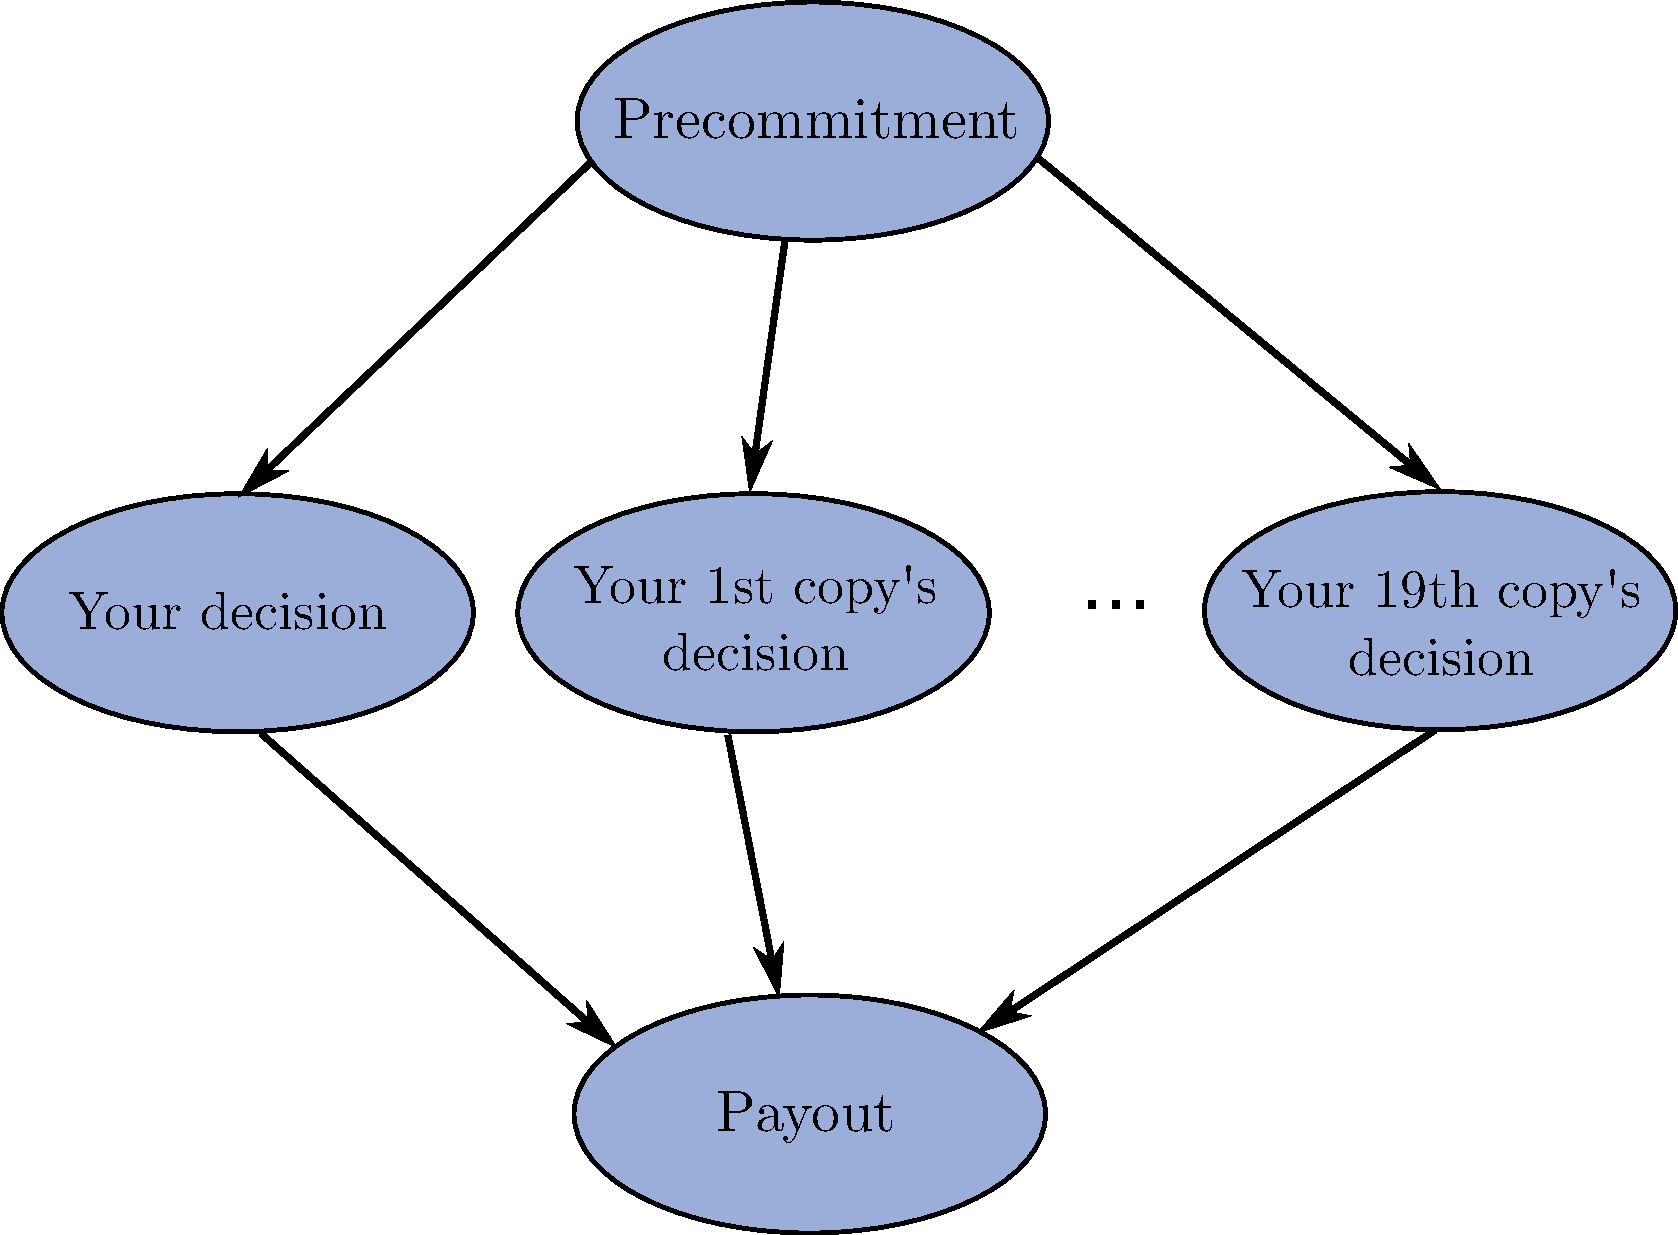
\includegraphics[width=3.46217in,height=2.59375in]{figs/precommitment-causal-graph}
    \caption{A causal graph representing the Donation game with copies and precommitment.}
    \label{precommitment-causal-graph}
\end{figure}


If CDT thinks that it will face some Newcomb-like problem where the copy
or model for prediction is created in the future, it would precommit to
make the same decision that acausal decision theories recommend (without
precommitment). Does that mean that CDT would have to make one
precommitment for each Newcomb-like problem (starting in the future)
that it will face with non-zero probability? Rather than patching its
behavior in each (future) Newcomb-like problem individually, CDT could
also make a more general self-modification. At time \emph{t}, it would
precommit to use the following alternative decision theory in the
future: do what I, at time step \emph{t}, would have precommitted to do
in the present situation
\parencite{Yudkowsky2010-ky,Soares2015-is,Meacham2010-pk}.
Such precommitment is not sufficient to generate the kind of
superrationality required for this paper: it does not cover Newcomb-like
problems that do not start in the future. That is, if the copies are not
created based on a future version of the agent, cooperation with them is
not covered by precommitment. Thus, CDT's precommitment does not imply
cooperation with agents in other parts of the multiverse. However, it
does suffice for a weaker version if we assume the Everett
interpretation of quantum physics (see section
\ref{multiverse-wide-superrationality-for-causal-decision-theorists}).

\hypertarget{lack-of-knowledge-is-evidential-power-part-ii-taking-a-step-back}{\subsection{Lack
of knowledge is evidential power, part II: taking a step
back}\label{lack-of-knowledge-is-evidential-power-part-ii-taking-a-step-back}}

CDT's precommitment only entails partial agreement with its rival
decision theories. Still, it is worth taking a closer look at
precommitment, as it leads us to another interesting dimension along
which decision theories can vary. Consider
\href{https://wiki.lesswrong.com/wiki/Counterfactual_mugging}{Counterfactual
mugging}, also known as ``the curious benefactor''
\parencite{Hintze2014-xs}:

\begin{quote}
\textbf{Counterfactual mugging.} Omega decides to play a game of heads
or tails with you. You are told that if the coin comes up tails, Omega
will ask you to give it \$100. If it comes up heads, Omega will predict
whether you would have given \$100 if the coin had come up tails. If
Omega predicts that you would have given it the money, it gives you
\$10,000; otherwise, you receive nothing. Omega then flips the coin. It
comes up tails, and you are asked to pay \$100. Do you pay?
\end{quote}

If you can precommit to giving the money before you learn about your
poor luck, you should do so. After all, this would render it
near-certain that Omega would give us \$10,000 if the coin came up
heads, at the mere cost of \$100 if it came up tails. By precommitting to
pay Omega, we thus gain
$0.5 \cdot \$ 10{,}000  - 0.5 \cdot \$ 100 = \$ 4{,}950$ in
expectation.

A CDT agent would, again, only precommit if Omega bases its decision on
a future version of the agent, whereas I (and many non-causal decision
theorists) would argue that we should precommit as long as the result of
the coin flip is unknown to us (even if Omega's model is based on a past
version of us).\footnote{In some versions of this problem, Omega has
  already flipped the coin when it approaches you. In those cases, you
  would still win by precommitting long after the coin has already
  landed, provided you are still uncertain about the result of the coin
  flip.} If we do so, we gain information that Omega thinks we give in,
and therefore that we will receive money in expectation. However, once
we learn that the coin came up tails, the ``winning'' move is to keep
the \$100. As before, the problem contains a harmful piece of
information -- although in this case an aspect of the environment, and
not a piece of information about the behavior of other agents, causes
trouble. If we got the chance, we would ``protect'' ourselves against
this piece of information by a precommitment, which renders that piece
of information harmless.

A similar reasoning applies to the Devious postal worker variant of the
donation game: If everyone precommits to cooperation irrespective of
what the postal worker's prediction says, then a negative prediction
about the other agents' behavior can no longer be self-fulfilling. Thus,
if you precommit to cooperating before the postal worker tells you about
the other agents' decisions, you have reason to expect more positive
news (assuming you correlate with the other agents).\footnote{Similar
  lines of reasoning about precommitment apply to thought experiments
  like the Newcomb's problem with transparent boxes
  \parencite{Drescher2006-ky}, retribution
  \parencite{Drescher2006-ky} and
  \href{https://wiki.lesswrong.com/wiki/Parfit\%27s_hitchhiker}{Parfit's
  hitchhiker} \parencite{Parfit1984-ne}.}

As is the case for CDT's precommitment in the previous section, this
leads to a more general self-modification that can be made instead of a
large number of individual precommitments for individual situations.
Specifically, we would (again) precommit to basing our decision in this
situation on what is good from the perspective of the state of knowledge
\emph{prior} to being given new information (like the result of the coin
toss). This is where
\href{https://wiki.lesswrong.com/wiki/Updateless_decision_theory}{updateless
decision theory} gets its name from, and I will call this feature of
decision theories
\href{https://casparoesterheld.com/2016/11/21/thoughts-on-updatelessnes/}{updatelessness}.
Contrary to what the term may suggest, it does not mean that we do not
react to new information at all, but rather that we do it in a different
way. Instead of updating the probabilities we assign to possible states
of the world and making the best decision based on that probability
distribution, we think about what we would have precommitted ourselves
to do in this situation. Usually, what we would have precommitted
ourselves to do is the same as what is then rational for us to do. For
example, if we take a bite from an apple and it tastes foul, we throw
the apple away. If you had to precommit to some action before learning
that the apple is foul, you would also precommit to throw the apple away
if it tastes foul (and to continue eating the apple if it tastes good).
Counterfactual mugging is one of the rare cases in which it does make a
difference.

Acausal decision theorists would precommit to be updateless about all
information they receive in the future. In essence, they would switch to
a decision theory that comes with updatelessness built-in (the most
notable one of them currently being
\href{https://wiki.lesswrong.com/wiki/Updateless_decision_theory}{updateless
decision theory}
\parencite{Benson-Tilsen2014-cv,Hintze2014-xs,McAllister_undated-ms}
itself). Thus, if you had been reasoning about (acausal) decision theory
including the possibility of self-modification correctly all along
(rather than only after learning about the experiment and its result),
you would actually cooperate in the Devious postal worker and give in to
Counterfactual mugging -- even without having precommitted to do so in
these \emph{particular} problems.

Some readers will no doubt already be familiar with updatelessness and
the arguments in favor of it. For those who have not, this may be a good
time to incorporate general updatelessness into their
decision-theoretical intuitions, as it is relevant for some of MSR's
implications (see sections
\ref{updateless-weights}
and \ref{schemes-of-causal-cooperation}).

As a side note, there are justifications of updatelessness that are not
based on precommitment and thus suggest that we should, e.\,g., give the
money in counterfactual mugging even if we previously have not thought
about precommitting to updatelessness. Ryan Carey lists a few in a
\href{https://agentfoundations.org/item?id=1199}{comment} on the
Intelligent Agent Foundations Forum. Benja Fallenstein
\href{http://lesswrong.com/lw/jkm/lzombies_lzombies/}{proposes}
\href{http://lesswrong.com/lw/jpr/sudt_a_toy_decision_theory_for_updateless/}{a
justification} based on ``logical zombies''. For other ideas, see
Armstrong \citeyear{Armstrong2011-sz} and
Drescher \citeyear{Drescher2006-ky}.\footnote{Also note that
  updateless behavior
  \href{https://casparoesterheld.com/2017/05/12/anthropic-uncertainty-in-the-evidential-blackmail/}{can}
  sometimes result from anthropic uncertainty even when applying the
  more classical evidential or causal decision theories.} However, these
are more complicated, non-obvious and not well-established. I thus opted
for limiting myself to the more straightforward precommitment-based
justification for updatelessness as discussed by Meacham~
\citeyear{Meacham2010-pk}, Fallenstein on~\href{http://lesswrong.com/lw/22m/selfmodification_is_the_correct_justification_for/}{LessWrong} and myself in a
\href{https://casparoesterheld.com/2016/11/21/thoughts-on-updatelessnes/}{blog post}
\parencite{Ahmed2012-ue}.

\hypertarget{reasons-and-correlations}{\subsection{Reasons and
correlations }\label{reasons-and-correlations}}

It is difficult to pin down the general principles of how the decisions
of different agents in different situations correlate. Indeed, I suspect
that the problem has no simple solution other than what is implied by
the general solutions to
\href{https://wiki.lesswrong.com/wiki/Naturalized_induction}{naturalized
induction} \parencite{Soares2014-hg,Soares2015-hu} and
decision theory.\footnote{Determining correlations between actions is
  similar to specifying the maxim corresponding to an action in
  \href{https://en.wikipedia.org/wiki/Categorical_imperative}{Kant's
  categorical imperative}. It
  \href{http://briantomasik.com/interpreting-the-categorical-imperative/\#If_everyone_did_what}{seems}
  \href{https://welovephilosophy.com/2013/01/07/choosing-a-kantian-maxim/}{that}
  nobody has a precise grasp of how the latter is supposed to be done
  and that this makes it difficult to apply the categorical imperative.
  However, the problem of specifying the maxim underlying one's action
  does not necessarily have a single correct solution. Determining
  correlations between your actions and that of others, on the other
  hand, follows from any solution to the problems of naturalized
  induction and decision theory. These solutions probably depend on
  priors, but it probably makes more sense to speak of them as having a
  correct solution.}

However, humans seem to have some good intuitions for how decisions
correlate, in part because understanding the correlations between
actions is a day-to-day activity. Imagine seeing your friend Anna being
wounded in her right arm one day. She uses her left arm to apply
bandages and call a doctor, who arrives a few minutes later and inspects
her right arm. A few days later, you see Bob being wounded in his left
arm. Based only on the experience from Anna's wound, what should you
reasonably expect to happen? Will Bob use his left arm to apply bandages
to his right one? Will \emph{Anna} apply bandages to \emph{her} right
arm? Or to Bob's? Will doctors come to Anna? Even after seeing just one
instance of a situation, we are often able to identify many of its
causal links and use this information to infer correlations with similar
situations. If we see the reasons for a decision from the inside, these
correlations become even clearer. If you are Anna and you apply bandages
to your right arm, you know that it is to stop the bleeding. Doing so
gives you no ``weird'' evidence -- it would not lead you to expect, say,
that people are generally likely to apply bandages to things
\parencite{Ahmed2014-ec,Almond2010-xn}.

In general, taking a particular action only because of some reason X
tells you nothing about whether agents who do \emph{not} care (or know)
about X will also take that action.

Importantly, superrationality itself falls under this general rule. That
is, if you do something for superrationality-related reasons, then this
does not tell you anything about how people who do not accept
superrationality would behave. As a trivial example, consider playing a
donation game against 19 people whom you all know to make fun of
superrationality whenever the opportunity avails itself. Attempting to
superrationally cooperate with those people seems rather fruitless.

While these considerations may seem trivial, alleged refutations of
acausal decision theories are often based on ignoring them or assuming
that the evidential thinker ignores them
\parencite{Ahmed2014-ec,Almond2010-xn}.

\subsubsection{Your back is not mine}\label{your-back-is-not-mine}

If the decisions of agents correlate or if each can determine what is
rational, then why can someone -- let us call him Dennis -- not just
determine that it is rational to benefit \emph{him} or his values?
Surely, if everyone just benefited Dennis, that creates the optimal
outcome for him. So, in a donation game with superrationality, perhaps
he should determine the rational policy to be ``cooperate, unless your
name is Dennis''?

This is clearly absurd. The specific reasons that lead Dennis to come up
with this strategy (and to abide by it) do not matter to his fellow
players, although each of them probably have self-serving reasons which
are analogous to those of Dennis. Dennis wants to achieve his own goals,
and this is done optimally if everyone cooperates while he alone
defects. However, this only makes it more likely that some other
participant -- let us call her Dana -- would reason, ``I want to
maximize my payoff; if I could determine everyone's choices, I would
want everyone but \emph{me} (Dana) to cooperate.''
\parencite{Drescher2006-ky}.

\subsubsection{Does accepting superrationality commit us to irrational
behavior in medical Newcomb
problems?}\label{does-accepting-superrationality-commit-us-to-irrational-behavior-in-medical-newcomb-problems}

One common objection to making decisions based on what our action
correlates with, rather than what our action causes, is that it seems to
imply irrational behavior in some cases
\parencite{Nozick1969-op}. In particular, reasoning from
correlation seems to fail in so-called \emph{medical Newcomb problems}.
An example is Yudkowsky's chewing gum
problem~\citeyear{Yudkowsky2010-ul}, which he describes as follows:

\begin{quote}
Suppose that a recently published medical study shows that chewing gum
seems to cause throat abscesses -- an outcome-tracking study showed that
of people who chew gum, 90\% died of throat abscesses before the age of
50. Meanwhile, of people who do not chew gum, only 10\% die of throat
abscesses before the age of 50. The researchers, to explain their
results, wonder if saliva sliding down the throat wears away cellular
defenses against bacteria. Having read this study, would you choose to
chew gum? But now a second study comes out, which shows that most
gum-chewers have a certain gene, CGTA, and the researchers produce a
table showing the following mortality rates:
\end{quote}

\begin{table}[h!]
    \centering
    \begin{tabular} {p{3cm} p{3cm}  p{3cm} }
        \toprule
        & CGTA present & CGTA absent \\
        \midrule
        Chew gum & 89\% die & 8\% die \\
        Don't chew & 99\% die & 11\% die \\
        \bottomrule
    \end{tabular}
\end{table}

\begin{quote}
This table shows that whether you have the gene CGTA or not, your chance
of dying of a throat abscess goes down if you chew gum. Why are
fatalities so much higher for gum-chewers, then? Because people with the
gene CGTA tend to chew gum and die of throat abscesses. The authors of
the second study also present a test-tube experiment which shows that
the saliva from chewing gum can kill the bacteria that form throat
abscesses. The researchers hypothesize that because people with the gene
CGTA are highly susceptible to throat abscesses, natural selection has
produced in them a tendency to chew gum, which protects against throat
abscesses. The strong correlation between chewing gum and throat
abscesses is not because chewing gum causes throat abscesses, but
because a third factor, CGTA, leads to chewing gum and throat abscesses.

Having learned of this new study, would you choose to chew gum?
\end{quote}

The causal graph of this problem is given in Figure~\ref{causal-graph-CGTA}.
Similar well-known decision problems of this kind are Solomon's problem
\parencite{Gibbard1978-nw,Eells2016-ym}, the Smoking lesion
\parencite{Eells2016-ym}, and the Psychopath button
\parencite{Egan2007-ey}.
\begin{figure}[h!]
    \centering
    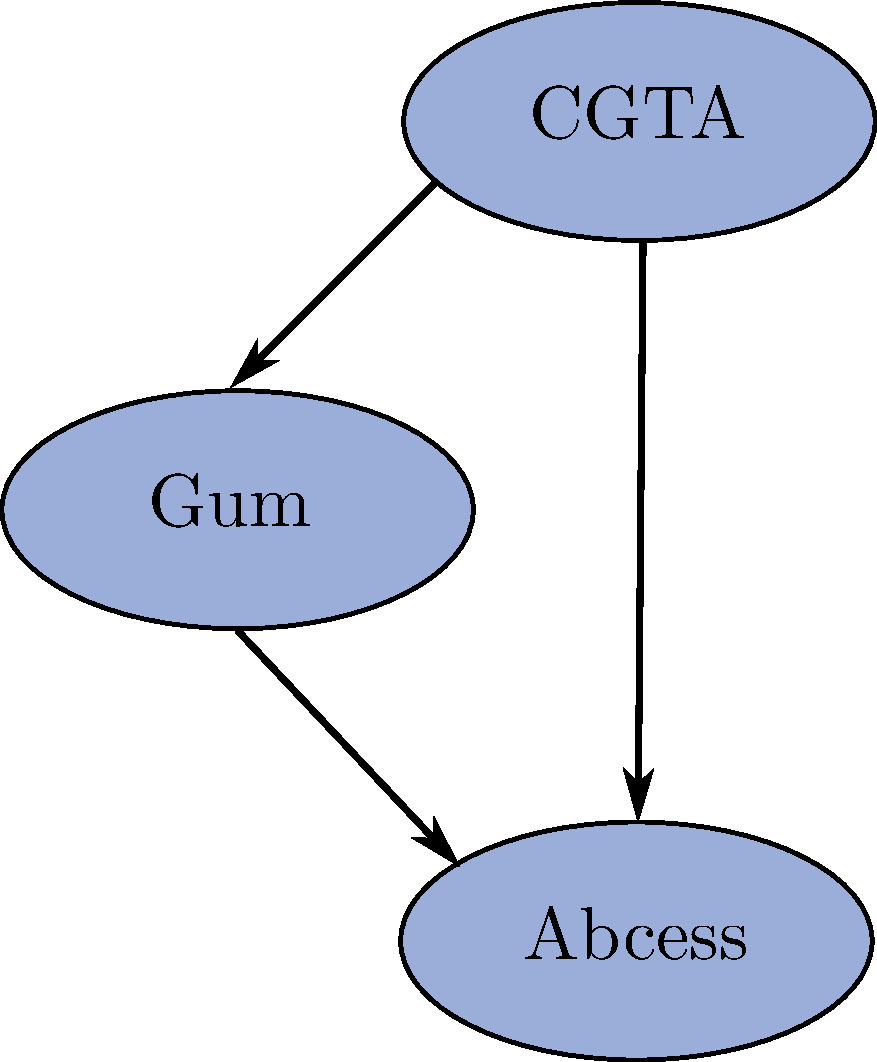
\includegraphics[width=1.95625in,height=2.48452in]{figs/causal-graph-CGTA}
    \caption{A graph representing the causal relationship
in the CGTA thought experiment.}
    \label{causal-graph-CGTA}
\end{figure}
%

Naive correlation-based reasoning suggests that we should still refrain
from chewing gum, since the act of chewing gum would be evidence that we
have the CGTA gene and thus throat abscesses. This strongly conflicts
with our intuition that we should chew gum to protect against the
abscesses. However, I will argue that this provides no convincing
argument against superrationality.

First, the correlation in the Chewing gum problem differs qualitatively
from the correlations between similar decision algorithms~\parencite{OesterheldTreutlein201X}.
%TODOLaTeX
In the Chewing gum problem (and
medical Newcomb problems in general), the correlation stems from a
causal relationship: our genes influence our decisions. Thus, the genes
and the decisions are correlated. The correlations of superrationality,
on the other hand, result from the similarity of the decision
algorithms. The reasoning behind cooperation does not involve a common
cause of all collaborators' decisions. Instead, the correlation may be
viewed as logical \parencite{Garrabrant2016-km}: if I
cooperate, then this implies that all copies of my decision algorithm
also cooperate. Figure \ref{two-types} illustrates the difference between
these two types of Newcomb-like problems. Because correlations in
medical and non-medical Newcomb-like problems differ qualitatively,
ignoring the correlations of our actions in the former does not mean we
should ignore them in the latter. In fact, in response to medical
Newcomb problems, philosophers have proposed a variety of decision
theories that behave in this exact way (Treutlein and Oesterheld,
unpublished). That is, they cooperate superrationally (and one-box in
Newcomb's problem) but chew gum in the Chewing gum problem. These
include Spohn's variation of CDT~\citeyear{Spohn2003-zf,Spohn2005-tm,Spohn2012-fo} and Yudkowsky's
timeless decision theory~\citeyear{Yudkowsky2010-ul}.

\begin{figure}[h!]
    \centering
    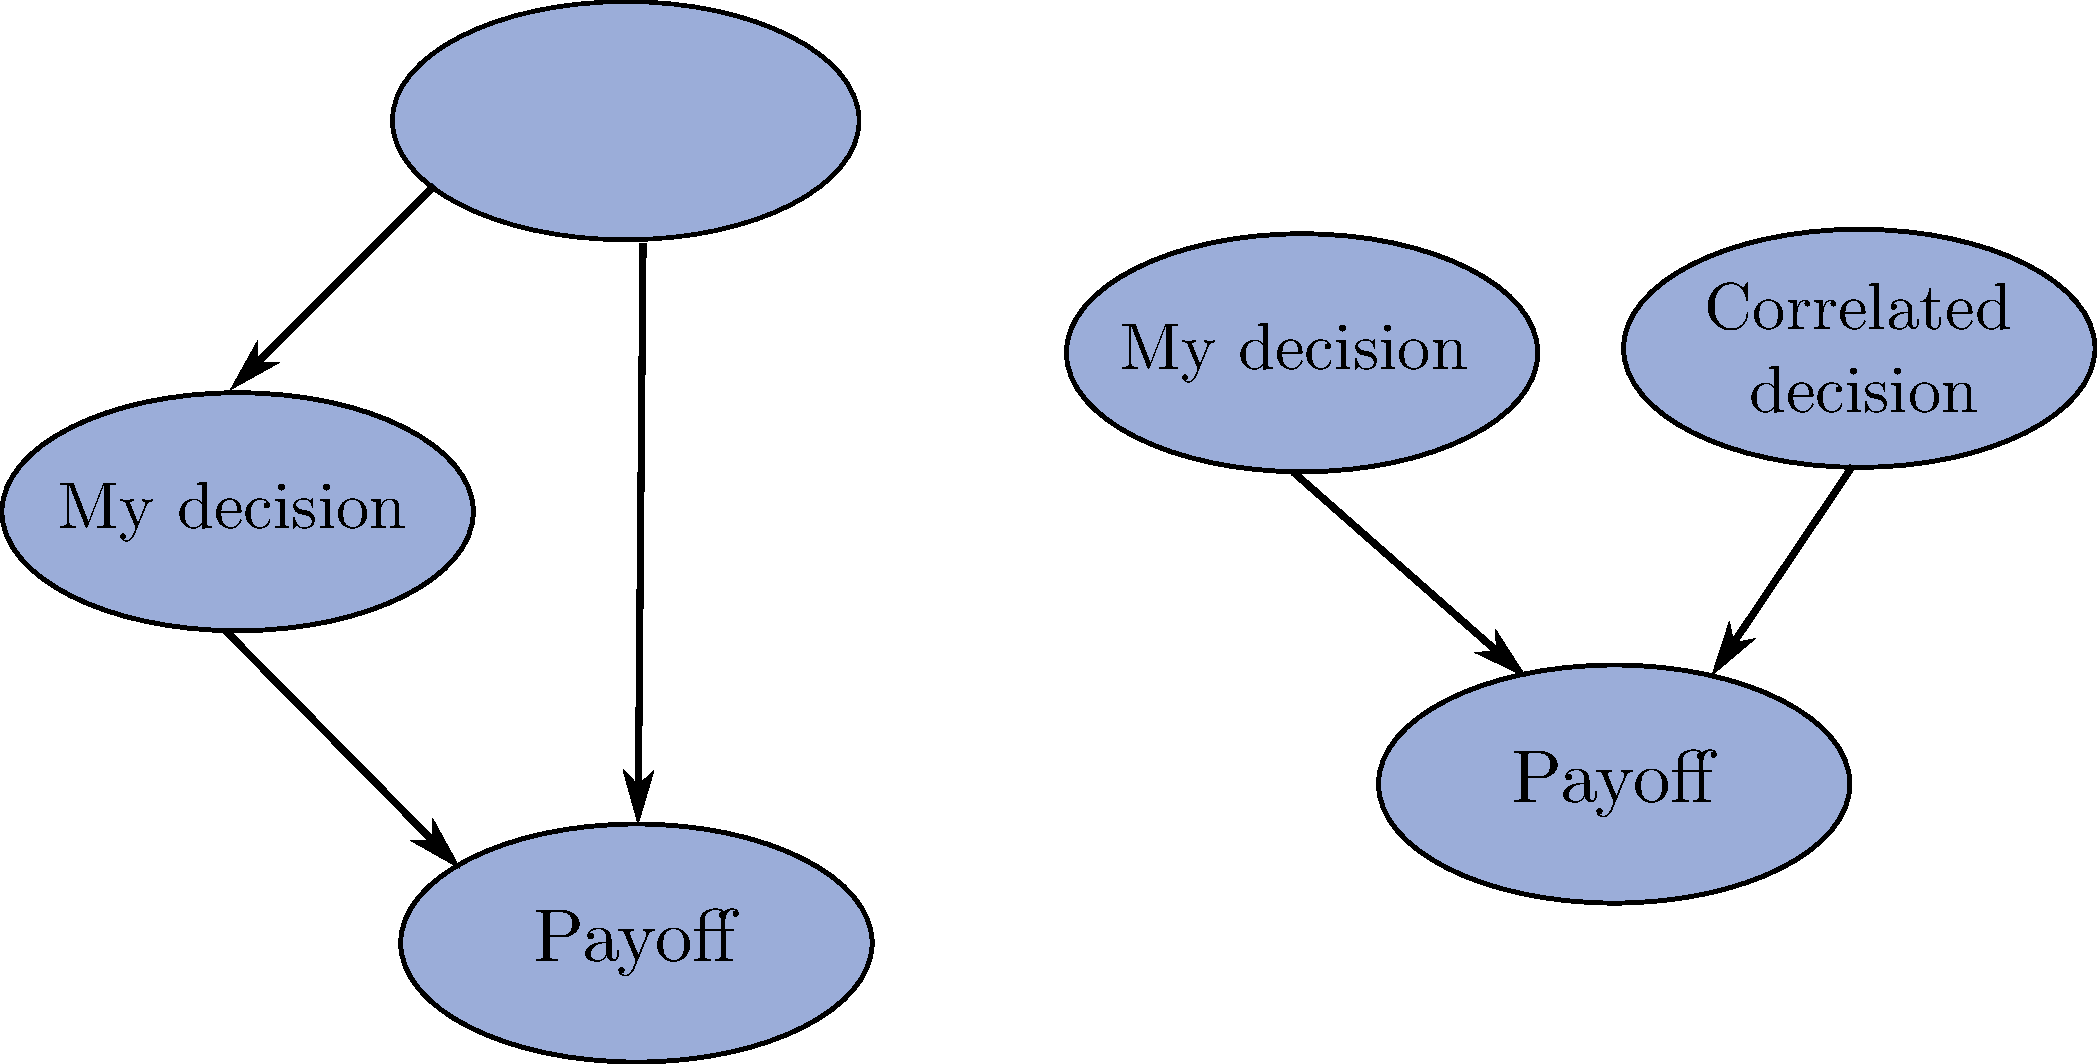
\includegraphics[width=4.1in]{figs/two-types}
    \caption{Generic causal graphs representing the two types of Newcomb-like decision problems. Medical Newcomb problems are illustrated on the left. Newcomb problems based on similarity between decision algorithms are illustrated on the right.}
    \label{two-types}
\end{figure}

Secondly, even purely correlation-based reasoning as done by EDT may
recommend chewing gum, depending on how the causal link from the CGTA
gene to chewing gum is believed to work. Given that people in the study
presumably did not know that chewing gum helps against throat abscesses,
it is plausible that CGTA causes people to intuitively desire chewing
gum. However, if learning about the study and applying EDT then causes
us not to chew gum, it does not tell us anything about whether having
the CGTA gene would have caused us to do the opposite. Similarly, if you
know that a sprinkler has watered the lawn, observing that the grass is
wet is no evidence that it has also rained (see Figure
\ref{tickle-defense}). The sprinkler already explains why the lawn is wet,
so you do not need rain as an additional explanation
\parencite{Ahmed2014-ec}.


\begin{figure}[h!]
    \centering
    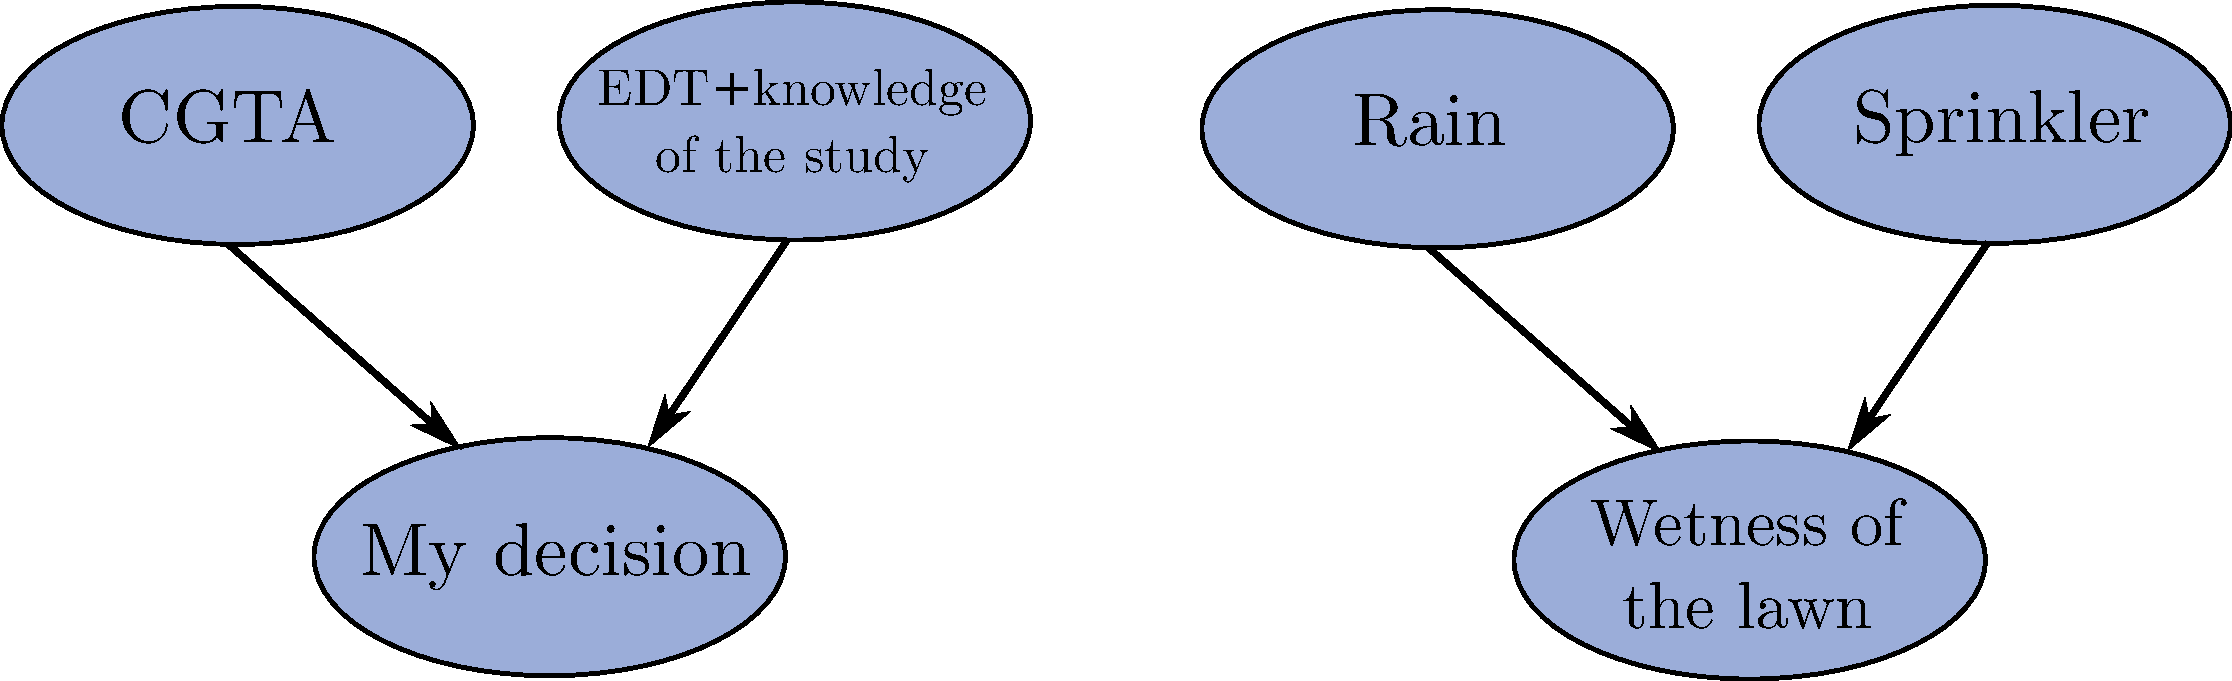
\includegraphics[width=4.09792in,height=1.27975in]{figs/tickle-defense}
    \caption{If you decide not to chew gum after applying EDT
to your knowledge of the study, it may tell you as much about whether
you have the CGTA gene as seeing a lawn watered by a sprinkler tells you
about whether it has rained.}
    \label{tickle-defense}
\end{figure}

\hypertarget{are-the-correlations-strong-enough}{\subsection{Are the
correlations strong enough?}\label{are-the-correlations-strong-enough}}

In most thought experiments in decision theory, it is assumed that the
other agents are near-copies of ours. The problems presented in this
paper are no exception. However, in any real-world setting, most agents
are not close copies of ours. We should therefore expect correlations to
be much less than perfect.

Luckily, the total number of agents in the multiverse is probably so
vast\footnote{In fact, most multiverse theories contain infinitely many
  agents. This leads to some additional complications, discussed in
  section \ref{infinite-ethics}.} that the correlations between ourselves and any
\emph{individual} agent need not be very large\footnote{Decision
  theorists have picked up on the point that large numbers of agents can
  bring out the differences between CDT and EDT in realistic cases. In
  particular, large elections are often mentioned as such a case
  \parencite{Ahmed2014-ec}.} (see section
\ref{many-agents}). Because many
agents probably don't know about superrationality, we may assume that
99.99\% of the agents do not correlate with us at all. In this case,
cooperation with the rest still pays off if we believe that our
correlation with the others is non-negligible and positive. It does not
matter that we inadvertently benefit many ``free riders''. For example:
if our cooperation makes it 1\% more likely that each of these
correlated agents also cooperates, then if there are ``only'' a billion
of them, we can expect 10 million more to cooperate if we
cooperate.\footnote{Note that this is usually not an instance of
  \href{https://wiki.lesswrong.com/wiki/Pascal\%27s_mugging}{Pascal's
  mugging}, although the underlying mathematical mechanism (multiplying
  very small numbers with very large numbers) is similar. Whereas in
  Pascal's mugging, a big reward outweighs the low probability assigned
  to it, multiverse-wide superrationality (MSR) involves a low
  probability being outweighed by the large number of near-independent
  instances of that probability. The positive result occurs with a high
  probability as long as the other agents' decisions of whether to
  cooperate are mostly independent of one another. For comparison,
  imagine drawing balls out of a box containing 1,000,000 balls. You are
  told that the probability of drawing a blue ball is only 1/1,000 and
  that the probabilities of different draws are independent. Given this
  information, you can tell with a high degree of certainty that there
  are quite a few blue balls in the box. Multiverse-wide correlations
  between agents thus becomes much more important to consider than the
  correlations in smaller scale problems like the donation game, unless
  we are skeptical of some of the underlying assumptions.}

\subsubsection{Correlation only with close
copies?}\label{correlation-only-with-close-copies}

Some might think that they are uncorrelated with everyone else apart
from very close copies of themselves. Because such near-copies would
likely share their utility function to a large extent, there is no need
to cooperate with them (although coordination
\protect\hyperlink{notes-on-superrational-coordination}{m}a\protect\hyperlink{notes-on-superrational-coordination}{y}
\protect\hyperlink{notes-on-superrational-coordination}{b}e useful,
depending on the utility function, see section
\ref{notes-on-superrational-coordination}). While the lack of formalized and
agreed-upon solutions to decision theory and naturalized induction
\parencite{Soares2014-hg,Soares2015-hu} makes it difficult
to draw definitive conclusions on such matters, I am nevertheless
skeptical of this objection to MSR. It seems to me that decision
theories, at least as people currently conceive of them, are compatible
with very large sets of possible minds. That is, if an agent uses, say,
evidential decision theory, it can still use all kinds of different
mechanisms for assigning conditional probabilities and, most
importantly, it can still have all kinds of values (see section
\ref{orthogonality-of-instrumental-rationality-and-values}).

\hypertarget{negative-correlations}{\subsubsection{Negative
correlations?}\label{negative-correlations}}

There is another interesting objection about correlation strength that
could be raised: perhaps we should expect to correlate \emph{negatively}
with some agents in the multiverse, such that cooperation can even do
some harm (beyond the opportunity costs connected to it) as it makes
some other agents more likely to defect. While interesting, I do not
find this reason against superrational cooperation very convincing,
either.

First, we have to consider what negative correlation means. Let's say
you currently think that roughly 0.1\% of evolved agents in the
multiverse who have thought about MSR decide to cooperate. Now, you
learn of one randomly chosen agent that she cooperates. The intuitive
response is to increase the 0.1\% estimate, if only slightly (depending
how confident you were in your initial estimate). If this agent were
\emph{negatively} correlated with the others, then upon learning that
this one agent cooperated, you would adjust your estimate of how many
agents cooperate \emph{downward}.

Such a reaction seems implausible given our state of knowledge. Surely,
there are a few eccentric agents who have superrationality-related
algorithms similar to mine, yet choose to somehow invert the output of
these algorithms. But such algorithms make little sense from an
evolutionary point of view and so I don't expect them to be very common
in the multiverse.

It may seem that agents have an incentive to become negatively
correlated (via self-modification), thereby enabling them to defect and
make everyone else cooperate. However, there are various problems with
this idea. For one, to be able to correlate negatively with the other
agents it seems as though one would have to find out about their
decision and then do the opposite, which appears to be difficult.
Furthermore, self-modification also commits us to cooperate more when
the others defect -- an agent committed to unconditional defection does
not correlate with anyone else.

The intuition underlying the self-modification idea is that by
self-modifying to be negatively correlated, we can acausally determine
the others' decisions. But I do not think this works in the relevant
way. When you modify your decision algorithm, you lay your power into
the hands of the new algorithm. This means you cannot, for example,
self-modify to some decision algorithm A that does the exact opposite of
what everyone else is doing, and then defect -- unless A is already
defecting on its own. Thus, you cannot determine everyone else to
cooperate unless you are already correlated with them. Similarly, you
cannot commit to output the 100th digit of $\pi$, and then return 6 anyway
to acausally determine the value of $\pi$. However, if you are already
correlated with the 100th digit of $\pi$, you can logically determine its
value. For instance, if Omega predicts your behavior and then tells you
that if you raise your arm, the 100th digit of $\pi$ will be 7 and if you do
not it will be 1, you can determine the 100th digit of $\pi$. Of course,
these stop working once you know what the 100th digit of $\pi$ is.

As a last point, self-modification does not seem to add anything to
direct defection (without self-modification). To see why, let us
consider the two kinds of agents that are not yet negatively correlated
with the others. The first agent is not correlated with others before
self-modification, and therefore has no reason to self-modify. He can
just defect directly, without adopting a weird decision theory that is
about doing the opposite of what someone in some other part of the
multiverse is doing. The second agent is (positively) correlated with
others before self-modification. Her problem is that if she
self-modifies, others will do so as well, which gives her evidence that
a lot more defection is happening than if she would cooperate.

Another relevant point is that there is a sharp upper bound to the
amount of negative correlation that can exist within a group of agents.
Imagine agents A, B, and C, whose decision to cooperate we model as a
random variable with the two values 1 (for cooperation) and 0 (for
defection). Let us say A is perfectly negatively correlated with B and B
is perfectly negatively correlated with C. A is then perfectly
\emph{positively} correlated with C. So, even among just three agents,
not all correlations can be perfect and negative. On the other hand, the
pairwise correlations may well all be perfect and \emph{positive}. To
study this further, we move from correlations to
\href{https://en.wikipedia.org/wiki/Covariance}{covariances},
because they
\href{https://en.wikipedia.org/wiki/Covariance\#Properties}{can}
be meaningfully added up. In general, we
\href{https://casparoesterheld.files.wordpress.com/2017/01/lowerboundavgcov.pdf}{can
derive} a lower bound of \(- \frac{1}{4(n - 1)}\) for the average
covariance between pairs of agents from any set of \(n \geq 2\) agents
(excluding ``pairs'' of one and the same physical agent), if cooperation
is seen as a binary
\href{https://en.wikipedia.org/wiki/Random_variable}{random}\footnote{Here
  ``random'' is, of course, meant in the
  \href{https://en.wikipedia.org/wiki/Bayesian_probability}{Bayesian
  sense}. That is, the behavior of other agents is random in the sense
  that we do not know it, not in the sense of arising
  non-deterministically.}
\href{https://en.wikipedia.org/wiki/Random_variable}{variable}.
If the agents are all perfectly correlated, then all covariances are at
most \(\frac{1}{4}\), so the \emph{upper} limit for the average
covariance is also \(\frac{1}{4}\).
\href{https://en.wikipedia.org/wiki/Mediocrity_principle}{Unless
we have reason to believe that we are special}, i.\,e. that our
covariance with the others falls far below the average covariance
between two agents, this suggests that especially for very large numbers
of agents \(n\), our possible acausal impact under the assumption of
only positive covariances can be much larger than that of negative
covariances. In fact, the covariances of the average agent cannot add up
to something below \(- \frac{1}{4}\) regardless of the number of agents.
In contrast, they can be as high as \(\frac{1}{4}(n - 1)\) for positive
covariances. If we
\href{https://casparoesterheld.com/2016/10/21/environmental-and-logical-uncertainty-reported-environmental-probabilities-as-expected-environmental-probabilities-under-logical-uncertainty/}{view
the covariances as uncertain}, this suggests a prudential argument in
favor of assuming positive covariances to dominate over negative ones,
given that our acausal influence is so small under the opposite
assumption. However, the details of this argument (and whether it works
at all) depend on our ``meta-probability distribution'' over
covariances.

\hypertarget{the-relative-importance-of-superrational-cooperation-an-example-calculation}{\subsection{The
relative importance of superrational cooperation: an example
calculation}\label{the-relative-importance-of-superrational-cooperation-an-example-calculation}}

Looking at a single decision, how do the benefits from superrational
cooperation compare with the opportunity costs? Although we need to make
some unrealistic assumptions (such as exact symmetry of the decisions
faced by all the agents) in order to calculate this value, it is
nevertheless worth an attempt, if only for the purpose of illustration.

We assume that there are \(n\) superrational agents whose decisions in
donation games are perfectly correlated; that is, either all of them
cooperate or all of them defect. Realistically, many more agents'
decisions will correlate weakly with ours, while only very few
correlations will be perfect. However, the implications of many weak and
a few strong correlations are similar. For simplicity, we assume that
the goals of the agents are orthogonal to each other, i.\,e. that if
someone benefits it is neutral in expectation to any other value system.
All of them have values that can benefit from behavior in other
universes to the same extent.

The \(n\) agents face the decision between a) generating \(b_{u}\)
\href{https://en.wikipedia.org/wiki/Cardinal_utility}{cardinal},
\href{https://en.wikipedia.org/wiki/Social_choice_theory\#Interpersonal_utility_comparison}{interpersonally
comparable} utils (or utilons) for their own utility function and b)
generating \(b_{\text{other}}\) utils for \(k\) randomly chosen
superrationalists.

Choosing option a) makes everyone chose option a) and so only generates
\(b_{u}\) utils for us. Choosing option b) makes everyone choose option
b). Whenever someone (including ourselves) chooses option b), there is a
probability of \(\frac{k}{n}\) that we are among the beneficiaries.

Overall, if we and thus everyone else chooses option b), we receive \(n\frac{k}{n}b_{\text{other}} =
kb_{\text{other}}\) utils. Choosing option b) is therefore to be preferred if and only if
\begin{equation}
kb_{\text{other}} > b_{u}.
    \label{eq:preferred}
    % previously (*)
\end{equation}

This suggests that our own preferences have no priority over those of
other superrationalists in this decision. We only decide based on ``the
greatest good for the greatest number''. For instance, if \(k = 1\),
then we should choose option b) to help other value systems if
\(b_{\text{other}} > b_{u}\), i.\,e. as long as helping other value
systems can be done more efficiently than helping your own values. This
shows how important superrationality considerations can be. Whereas the
non-superrational agent maximizes only for its own value system, the
superrational agent maximizes for the value systems of other
superrational agents just as much as for their own.

Moreover, whether we cooperate depends only on the number of agents
whose cooperation is correlated with ours and not at all on the number
of agents that will defect. In this regard, multiverse-wide
superrational cooperation differs from most causal cooperation, where we
usually try to ensure that beneficiaries of our actions reciprocate
(unless we care about them intrinsically).

As mentioned already, this analysis is based on unrealistic assumptions
of perfect symmetry to highlight the relative importance of
superrationality considerations. We will now move on to more general,
potentially asymmetric cases.

\hypertarget{compromise-strategy}{\subsection{Compromise
strategy}\label{compromise-strategy}}

\subsubsection{Sharing gains from compromise in the face of
asymmetries}\label{sharing-gains-from-compromise-in-the-face-of-asymmetries}

We have so far only considered completely symmetrical situations,
wherein other agents faced the exact same decision problem as ourselves.
One could either choose to cooperate, which correlated with everyone
else's cooperation; or defect, which correlated with everyone else's
defection. Both cooperation and defection were associated (via the
correlation between agents) with particular outcomes. Based on these
correlations it was straightforward to choose the action that correlates
with the best outcome for ourselves (and also for everyone else). Of
course, in practice, compromise will not be this tidy. Specifically, we
will have to deal with asymmetrical decision problems. Consider the
following example:

\begin{quote}
\textbf{Superrational
\href{https://en.wikipedia.org/wiki/Fair_cake-cutting}{cake
cutting}.} You are playing a donation game with two fellow players
whose decision algorithms correlate strongly with yours. Unlike other
donation games, the currency in this game is cake, of which there are
two flavors -- vanilla and strawberry. Each player's utility grows in
linear proportion to how much cake they eat, and they all have taste
preferences that affect their total utility. Let's say you, player 1,
like vanilla twice as much as strawberry. Player 2, meanwhile, likes
strawberry four times as much as vanilla, and player 3 likes both
flavors equally. Each player currently owns different amounts of
strawberry and vanilla cake. You have one strawberry cake and one
vanilla cake, while player 2 has three vanilla cakes and player 3 has
one strawberry cake. (See Figure
\ref{Superrational-cake-cutting} for an illustration of
these circumstances.) You all know each other's taste preferences and
can send arbitrary fractions of your cakes to one another, but none of
you are allowed to communicate. You only get to send one box of cake to
each player, and you receive your boxes from them after you've sent
yours. What should you do?
\end{quote}

\begin{figure}[h!]
    \centering
    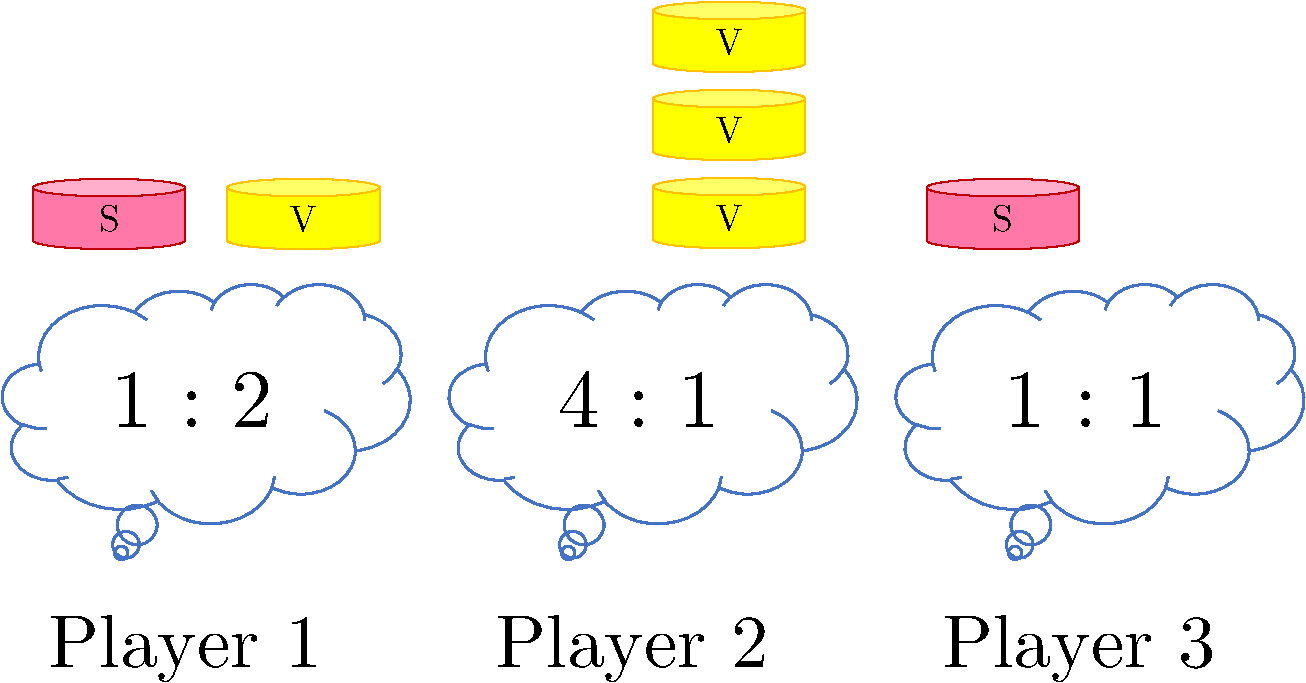
\includegraphics[width=4in]{figs/Superrational-cake-cutting}
    \caption{An overview of property and preferences in the Superrational cake cutting.}
    \label{Superrational-cake-cutting}
\end{figure}

First note that this problem is indeed one of superrational cooperation.
If causal decision theory is applied, then the dominant strategy for
each player is to keep all the cake -- but this would be a suboptimal
outcome for everyone. The players have two strawberry and four vanilla
cakes in total. If you could redistribute them so that player 1 has one
strawberry and two vanilla cakes, player 2 has one strawberry cake, and
player 3 has two vanilla cakes, everyone would be better off than
without any redistribution. However, there are an infinite number of
other possible (fractional) distributions that would also be better for
everyone. This makes it hard to decide among them.

One part of the problem is that it is unclear what our decisions
correlate with. If we send player 2 a piece of her preferred cake
(strawberry), can we expect to get some of our preferred cake (vanilla)
from her? If so, how much? If we could pin down the correlations and
assign probabilities to each combination of strategies -- i.\,e. to each
\href{https://en.wikipedia.org/wiki/Strategy_(game_theory)}{strategy
profile} -- conditional on any of our actions, we could choose the
action that maximizes expected utility (the exact formulation of which
depends, of course, on our decision theory). But even if the agents know
that they have very similar (or even identical) decision algorithms, the
asymmetries make it hard to assign these probabilities.

Another perspective on the problem is that asymmetries make it unclear
who ``deserves'' how much. In the symmetrical situations it was always
clear that everyone should get the same, but this is different in
superrational cake-cutting.

It is useful to view the symmetry of a compromise problem as a
non-binary property. For example, a donation game in which one player
gains slightly more than the others from cooperating may still be
symmetric enough to make it obvious what the right decision is.

\hypertarget{the-compromise-problem}{\subsubsection{The compromise
problem}\label{the-compromise-problem}}

In order to solve the problem of superrational compromise in asymmetric
situations, we will treat compromise as a game-theoretical problem. Note
that this requires basic knowledge of game theory; for an introduction
see, e.\,g. \citeyear{Osborne2004-ui}. Formally, a game
consists of

\begin{itemize}
\item
  a finite set of players \(P = { p_{1},\dotsc,p_{n}}\),
\item
  for each player \(p_{i}\), a set of actions \(A_{i}\),
\item
  for each player \(p_{i}\) a utility function
  \(u_{i}\colon A_{1} \times \dotsm \times A_{n} \rightarrow \mathbb{R}\), where
  \(\mathbb{R}\) refers to the real numbers. 
\end{itemize}

Multiverse-wide superrational compromise is a game where \(P\) is the
set of correlated superrationalists, the utility functions \(u_{i}\)
represent their preferences, and the sets of possible actions \(A_{i}\)
represent the set of strategies a player can pursue in their part of the
multiverse. Note that the last aspect of the definition assumes that the
players' preferences are
\href{https://en.wikipedia.org/wiki/Von_Neumann\%E2\%80\%93Morgenstern_utility_theorem\#The_axioms}{von
Neumann-Morgenstern-rational} (vNM-rational), which is technically
useful and mostly non-controversial\footnote{One exception may be the
  axiom of continuity. It is violated by preferences with lexicality,
  which are commonly discussed in moral philosophy
  \parencite{Knutsson2016-kd}. However, if we drop the axiom
  of continuity,
  \href{https://casparoesterheld.com/2016/08/08/lexicographic-utility-functions/}{we
  can} still represent the preferences as a lexicographic utility
  function \parencite{Blume1989-fd,Fishburn1971-bx}.
  However, a treatment that includes lexicographic utility functions is
  beyond the scope of the present paper. Because in uncertain
  situations, a lexicographic utility function is usually equivalent to
  only maximizing the lexically highest values, we may nonetheless apply
  the present results by simply omitting all lexically lower values.}.

Our notation indicates that utilities are calculated deterministically
from action tuples. However, we will sometimes view the utilities
\(u_{i}(a_{1},\dotsc,a_{n})\) as random variables in the
\href{https://en.wikipedia.org/wiki/Bayesian_probability}{Bayesian
sense}. This is because we are usually uncertain about the implications
of the policies \(a_{1},\dotsc,a_{n}\), as well as the utility function
\(u_{i}\) itself, in the context of MSR.

Now, the question is which (potentially
\href{https://en.wikipedia.org/wiki/Strategy_(game_theory)\#Mixed_strategy}{mixed})
strategy \(\alpha_{i}\) any player \(p_{i}\) should choose. Note that we
are not looking for the (CDT-based) Nash equilibria of the game. We will
therefore have to move our focus from (Nash equilibrium-based)
\href{https://en.wikipedia.org/wiki/Non-cooperative_game_theory}{non-cooperative}
to
\href{https://en.wikipedia.org/wiki/Cooperative_game_theory}{cooperative
game theory}.

In principle, the optimal strategy \(\alpha_{i}^{*}\) can be determined
by applying one's decision theory. For example, if one were to use EDT,
then the optimal strategy is
$$
\argmax_{\alpha_{i}}\ \mathrm{E}\lbrack u_{i}(a_{1},\dotsc,a_{n})\mid \alpha_{i}\rbrack.
$$
As noted earlier, however, computing or optimizing the expected value
conditional on one's action directly is not feasible in situations of
asymmetric payoffs. To find the best action, we will therefore
approximate the above expected value maximization with some new
criterion, similar to how game theory has replaced expected value
maximization with Nash equilibria and other concepts.

We will therefore try to develop some new \emph{compromise utility
function} \(u^{*}\colon A_{1} \times \dotsm \times A_{n} \rightarrow \mathbb{R}\),
intended as a new criterion for choosing the optimal strategy. Because
the compromise utility function depends less on the specifics of the
problem, it will prove to be easier to reason about what the adoption of
some \(u^{*}\) tells us about what the other agents do. The optimal
\(u^{*}\) can then, under certain assumptions, tell us what action to
take. At least if our choosing \(u^{*}\) means that everyone else
chooses the same \(u^{*}\) (which is not necessarily the case), then
player \(p_{i}\) should implement the \(i\)-th strategy entry of
$$
\argmax_{(\alpha_{1},..,\alpha_{n}) \in A_{1} \times \dotsm \times A_{n}}\ \mathrm{E}\lbrack u^{*}(\alpha_{1},\dotsc,\alpha_{n})\rbrack.
$$
Once again, having a compromise \emph{utility function,} as opposed to
more general compromise \emph{preferences}, implicitly assumes that the
compromise preferences are also vNM-rational.

\hypertarget{cooperation-with-and-without-coordination}{\subsubsection{Cooperation
with and without
coordination}\label{cooperation-with-and-without-coordination}}

In a way, \(\argmax_{(\alpha_{1},..,\alpha_{n}) \in A_{1} \times \dotsm \times A_{n}}\
\mathrm{E}\lbrack u^{*}(\alpha_{1},\dotsc,\alpha_{n})\rbrack\) is the optimal plan on the assumption
that everyone will follow it. With practical degrees of correlations, however, we cannot assume that
everyone will arrive at the same plan, especially if multiple plans have
the same compromise utility. In MSR, it is especially unlikely that
everyone will arrive at the same plan, as superrational collaborators
have different states of knowledge about the multiverse and each others'
value system.

A perfect plan may have catastrophic results if it is not accurately
followed by everyone involved. Specifically, plans are risky if the
utility of one player's action hinges on another player's action because
such plans assume the ability to coordinate. Hence, it is useful to look
at a class of utility functions where coordination plays no role.

We say that a utility function \(u_{i}\) \emph{(additively) decomposes
into local utility functions}
\(\{ u_{i,j}\colon A_j \rightarrow \mathbb{R}\}_{j = 1,\dotsc,n}\) if
$$
u_{i}(a_{1},\dotsc,a_{n}) = \sum_{j=1}^n u_{i,j}(a_{j}).
$$

Intuitively speaking, \(u_{i}\) decomposing into local utility functions
means that any player \(p_{j}\) has a very direct impact on \(p_{i}\)'s
utility, such that when \(p_{j}\) attempts to benefit \(p_{i}\) she need
not think about what other players do.

In game theory as it is usually applied to interactions between agents
on Earth, the assumption of additive decomposition of utility functions
would be a severe limitation: if agents interact with each other
physically, then, of course, the impact of an action often depends on
the other players' actions. As examples, consider some of the classic
games studied in game theory, such as
\href{https://en.wikipedia.org/wiki/Battle_of_the_sexes_(game_theory)}{Bach
or Stravinsky} or
\href{https://en.wikipedia.org/wiki/Chicken_(game)}{Chicken}.

In the problem of multiverse-wide compromise, on the other hand, there
is probably no causal interaction between the actions of agents in
different parts of the multiverse. Additive decomposition of utility
functions is thus a more natural assumption in this context. That said,
issues of coordination can still arise in the utility function itself.
As an example, consider a utility function that wants there to be at
least one (dis-)proof of the
\href{https://en.wikipedia.org/wiki/Riemann_hypothesis}{Riemann
hypothesis} somewhere in the multiverse, but does not care about the
existence of further, redundant proofs. This utility function does not
decompose additively; whether I benefit this utility function by proving
the Riemann hypothesis depends on whether someone else is already
working on a proof. Other, perhaps more realistic, examples of ethical
notions that do not decompose into local utility functions are (partial)
\href{https://en.wikipedia.org/wiki/Average_and_total_utilitarianism}{average
utilitarianism} and potentially
\href{https://en.wikipedia.org/wiki/Biodiversity}{biodiversity}.
However, many other plausible utility functions (e.\,g., total
utilitarianism) do fulfill the above condition.

If some of the utility functions in a game do not decompose into local
utility functions, we will call the game a \emph{coordination
problem}\footnote{This differs somewhat from more standard
  game-theoretical definitions of coordination. For a discussion of the
  relationship, see \parencite{Oesterheld2017-lt}.}.
Theoretically, the following arguments also work for coordination games,
but they are much more robust and practically applicable in problems
that require little or no coordination. This topic will be discussed
further in section
\ref{notes-on-superrational-coordination}.

\subsubsection{Harsanyi's aggregation
theorem}\label{harsanyis-aggregation-theorem}

Although we do not yet know how and to what extent, we know that our
compromise utility function \(u^{*}\) should incorporate the utility
functions \(u_{1},\dotsc,u_{n}\) but not be sensitive to anything else. The
following assumption captures these attitudes:

\vspace{3mm}

\begin{assumption}
\label{ass:compromise_util}
Let P and Q be probability distributions over outcomes \(A_{1} \times
\dotsm \times A_{n}\) such that \(\mathrm{E}_{P}\lbrack u_{i}(a_{1},\dotsc,a_{n})\rbrack \geq
\mathrm{E}_{Q}\lbrack u_{i}(a_{1},\dotsc,a_{n})\rbrack\) for \(i = 1,\dotsc,n\).\footnote{This notation --
    viewing the lotteries as probability distributions over action vectors -- is a bit unnatural,
    and stems from the lack of an intermediate step of world states or histories between action
    vectors and utilities in our notation. If we extended our notation with such an intermediate
    step, then the lotteries would be over states of the world rather than action vectors. Although
the proofs also work with action vectors, it may help to think of the lotteries as being over
histories.} That is, all players like P at least as much as Q. Then \(\mathrm{E}_{P}\lbrack
u^{*}(a_{1},\dotsc,a_{n})\rbrack \geq \mathrm{E}_{Q}\lbrack u^{*}(a_{1},\dotsc,a_{n})\rbrack\), i.\,e. the
compromise utility function also values \(P\) at least as highly as \(Q\).
\end{assumption}

We could view this assumption as a decision to limit ourselves to a
particular class of compromise utility functions -- a decision that
makes our superrational collaborators limit themselves to the same
class. In terms of expected value for ourselves, this is a good
decision. It basically does not tell us anything other than that we do
not want to pay anything to switch from P to Q if everyone likes P at
least as much as Q.

We furthermore introduce the notion of utility function equivalence: two
utility functions \(u\) and \(v\) are equivalent, written as
\(u \sim v\), if they imply equal behavior. For the
\href{https://en.wikipedia.org/wiki/Cardinal_utility}{cardinal
utility functions} discussed here, this is the case if one arises from
positive affine transformation of the other, i.\,e. if \(u = av + b\) for
some \(a \in \mathbb{R}_{> 0}\) and \(b \in \mathbb{R}\).

Assumption~\ref{ass:compromise_util} does not seem especially strong, but it turns out that it
suffices for a significant result regarding the shape of the compromise utility function. It is
essentially a version of Harsanyi's aggregation theorem (\cite{Harsanyi1955-ou}; see also
\cite{Peterson2017-pa}, section 13.4 for an introduction).\footnote{Interestingly, the proof of the
    aggregation theorem given in \citeyear{Harsanyi1955-ou} contains an error. However, since then
    a few alternative, correct proofs have been published
    \parencite{Fishburn1984-zh,Border1985-mw,Hammond_undated-bp}.}

\begin{theorem}
\parencite{Resnik1983-hl,Fishburn1984-zh} Let \(u^{*}\) be
a compromise utility function for \(u_{1},\dotsc,u_{n}\) that satisfies
Assumption B. Then there are weights
\(\lambda_{1},\dotsc,\lambda_{n} \in R_{\geq 0}\) such that
\begin{equation}
    u^{*} \sim \sum_{i=1}^n\lambda_{i}u_{i}.
    %previously (**)
    \label{eq:weights}
\end{equation}
    \label{th:compromise}
\end{theorem}

Note that the \(\lambda_{i}\) are not unique. Also, not all weight
assignments consistent with Eq.~\eqref{eq:weights} or Assumption~\ref{ass:compromise_util} have only positive
weights. In particular, if \(u_{i} = u_{j}\) for some \(i \neq j\), we
can decrease \(\lambda_{i}\) by an arbitrary constant \(C\) if we
correspondingly increase \(\lambda_{j}\) by \(C\), and end up with the
same utility function
\parencite{Resnik1983-hl,Fishburn1984-zh}. If
\(C > \lambda_{i}\), we arrive at an equivalent utility function that
assigns negative weights.


\begin{theorem}
Let \(u_{1},\dotsc,u_{n}\) each decompose into local utility functions \(\{{ u}_{i,j}\colon A_{j} \rightarrow
\mathbb{R}\}_{j = 1,\dotsc,n}\).  Then a compromise utility function \(u^{*}\) that satisfies
Assumption~\ref{ass:compromise_util} relative to \(u_{1},\dotsc,u_{n}\) also decomposes into local
utility functions.
    \label{th:decompose}
\end{theorem}

\begin{proof}
Because of Theorem \ref{th:compromise}, it is 
\begin{equation*}
    \begin{split}
        u^{*}(a_{1},\dotsc,a_{n}) &= b + \sum_{i=1}^n\lambda_{i}u_{i}(a_{1},\dotsc,a_{n}) \\
                               &= b + \sum_{i=1}^n\lambda_{i}\sum_{j=1}^nu_{i,j}(a_{j}) \\
                               &= b + \sum_{j=1}^n\sum_{i=1}^n\lambda_{i}u_{i,j}(a_{j}) \\
                               &= \sum_{j=1}^n\Bigl(\frac{b}{n} +
                               \sum_{i=1}^n\lambda_{i}u_{i,j}(a_{j})\Bigr)\\
    \end{split}
\end{equation*}
for some \(b\) and weights \(\lambda_{1},\dotsc,\lambda_{n}
\in \mathbb{R}_{\geq 0}\). Thus, \(u^{*}\) decomposes into local utility functions
\begin{equation*}
\Bigl\{u_j^*\colon A_j \rightarrow \mathbb{R}\colon a_j \rightarrow \frac{b}{n} + \lambda_i
u_{i,j}(a_{j})\Bigr\}_{j = 1,\dotsc,n}.
\end{equation*}
\end{proof}
This is quite a convenient result. If indeed \(u_{1},\dotsc,u_{n}\) each
decompose into local utility functions, then each player \(p_{i}\) can
maximize \(u_{i}^{*}\) in her own part of the multiverse without having
to think about the precise actions of other players elsewhere in the
multiverse.

\hypertarget{how-to-assign-the-weights}{\subsubsection{How to assign the
weights}\label{how-to-assign-the-weights}}

Having argued that we should make our decisions based on a weighted sum
of the decisions of our superrational collaborators, the question is how
we should optimally assign the weights. Theorem~\ref{th:compromise} does not tell us much
about this. In fact, it even allows for the possibility of assigning
positive weight only to our own utility function. We will differentiate
two ways of assigning the weights: biased toward our own values, or
impartial. We will consider the two options in turn.

\paragraph{Biased compromise utility
functions?}\label{biased-compromise-utility-functions}

We start with the option of assigning the weights in a way that is
somehow biased toward our values. For example, we could assign higher
weights to utility functions that are more compatible with ours, and
lower weights to those that are not. Of course, this tells us that
agents with other value systems will do the same, i.\,e. assign weights in
a way that bias the resulting utility function toward their own values.

I will argue against assigning weights in a biased way and in favor of
impartial weights. This point is crucial for the strength of the
implications of MSR, because the more weight we assign to other utility
functions, the more our policies have to change in response to MSR.

In a way, the reasons against biased weights are merely an extension of
the reasons for cooperating in the first place. Let us say that in
response to MSR we assign some weight to the other agents' utility
functions but still largely maximize for our own values. Then gains from
further trade are left on the table. Because we still maximize for
different utility functions, we could trade again until all our
compromise utility functions approach some impartially weighted sum.

This line of reasoning is also supported by the standard ways in which
gains from trade arise. If everyone compromises with biased weights,
then this produces some gains from
\href{https://en.wikipedia.org/wiki/Comparative_advantage}{comparative
advantages} -- in situations where I have a large comparative advantage
to maximize for someone else's utility function, I will do so at the
cost of not maximizing for my own values. In return, others do the same.
But if the comparative advantages are too small, then we miss out on
gains from trade. Consider an example with two superrational
collaborators. For simplicity, we will assume them to be in symmetrical
situations at the time of compromise, such that the only plausible
neutral compromise would give the same weight to each of the two utility
functions. Both may, at some point, face the choice between taking a
utility of \(x\) for themselves and giving \(x + \varepsilon\) to the
other, where \(x\) and \(\varepsilon\) are any positive real numbers. In
such a situation both have a comparative advantage to help the other's
values. But if \(\varepsilon\) is very small, the comparative advantage
is very small, too. So, if they assign more weight to their own utility
functions, there is some \(\varepsilon\) such that they choose to
maximize their own utility functions and thus miss out on the gains from
trade.

While I am moderately confident that all compromises with biased weights
are Pareto-suboptimal, I do not, at this point, have a formal proof of
this statement. That said, the above example at least shows that such
compromises yield collectively
\href{https://en.wikipedia.org/wiki/Von_Neumann\%E2\%80\%93Morgenstern_utility_theorem\#The_axioms}{vNM-irrational}
behavior. Furthermore, section
\ref{the-relative-importance-of-superrational-cooperation-an-example-calculation} showed that, at least in symmetrical idealized
scenarios, prioritizing one's own values does not achieve the best
results.

I should note that impartial weights do not imply that I should be
equally likely to find myself maximizing for my own values as any of my
superrational collaborators. For example, if you are very uncertain of
the content of some value system, then it will not influence your
decisions as much, even if you assign a high weight to that value
system.

\paragraph{Neutral compromise utility
functions}\label{neutral-compromise-utility-functions}

We have argued that after an optimal compromise, each player should
judge their action roughly by the same impartial criteria. Hence, we now
have to look for a way of assigning the weights in a neutral way.

Harsanyi himself proposes -- albeit in
the context of social welfare rather than trade -- to simply give equal
weight to all utility functions, which is equivalent to removing the
weights altogether~\parencite{Harsanyi1979-ac}. Besides the argument of ``equal treatment'', it can
be backed by an
\href{https://en.wikipedia.org/wiki/Original_position}{original
position} argument
\parencite{Harsanyi1953-mj,Harsanyi1955-ou,Freeman2016-kg}.
From an original position, i.\,e. a perspective from which we do not yet
know which position in the multiverse we will take, how many resources
will be at our disposal, etc., it seems reasonable to give equal weight
to all utility functions. Updatelessness gives this argument some
additional appeal, as it asks us to make our decisions from a similar
perspective.

However, there are various problems with maximizing unweighted
aggregated utility. One is that it is based on interpersonal comparisons
of utility. In Harsanyi's words, it assumes that ``all individuals'
utility functions \(u_{1},\dotsc,u_{n}\) are expressed in equal utility
units (as judged by individual \(j\) on the basis of interpersonal
utility comparison)''.\footnote{Note that none of the previous arguments
  were based on interpersonal comparisons of utility.} Such comparisons,
however, are highly controversial
\parencite{Hammond1991-rj,Binmore2007-da}. Recall that the
cardinal utility functions postulated by the
\href{https://en.wikipedia.org/wiki/Von_Neumann\%E2\%80\%93Morgenstern_utility_theorem}{von
Neumann-Morgenstern utility theorem} are only determined up to positive
affine transformation. This means that if a utility function \(u\)
represents an agent's preferences, then so do \(100 \cdot u\) and
\(0.01 \cdot u\). None of the three is in some way the more natural
choice for representing the agent's utility function. Whereas positive
affine transformations do not alter an agent's behavior in choosing
\href{https://en.wikipedia.org/wiki/Von_Neumann\%E2\%80\%93Morgenstern_utility_theorem\#Set-up}{lotteries},
they do change the behavior implied by the aggregate of multiple such
functions. In Superrational cake cutting, we specify the utility
functions (or, as they are sometimes called in
\href{https://en.wikipedia.org/wiki/Fair_cake-cutting}{fair
cake-cutting}, subjective value functions) of each agent up to positive
affine transformation by specifying the trade rates between units of
strawberry and vanilla cake. For example, the third player has a 1:1
trade ratio, the second has a 4:1 trade ratio. To simplify notation, let
\(s_{i}\) and \(v_{i}\) be amounts of strawberry and vanilla that
\(p_{i}\) receives under some action profile. Then the second player's
utility function could be \(u_{2}(s_{2},v_{2}) = 4s_{2} + v_{2}\) and the
third player's utility function could be written as
\(u_{3}(s_{3},v_{3}) = s_{3} + v_{3}\). If one wanted to maximize
aggregate utility \(u_{2} + u_{3}\), then \(u_{2}\) would effectively
receive far more weight than \(u_{3}\). If
\(u_{2}(s_{2},v_{2}) = 400s_{2} + 100v_{2}\), this bias toward \(u_{2}\)
would be even worse.

Because utility functions come in different versions depending on their
scale, we still need to find a satisfactory way of normalizing the
utility functions, i.\,e. to pick one out of a whole class of equivalent
utility functions. This task is actually equivalent to assigning a
weight to a given member of each class. Thus, removing the weights and
relying on interpersonal comparison of utility can be seen as merely
passing the buck from assigning weights to choosing the scale of the
utility function.

One common approach to interpersonal comparison of utility is range
normalization \parencite{Isbell1959-ql,Hausman1995-ry}. That
is, the utility functions are chosen in such a way that their maximum is
1 and their minimum is 0 (using no additional weight).\footnote{There is
  a technical problem with utility functions that do not assume a
  highest/lowest value at all. If they are nonetheless bounded, the
  \href{https://en.wikipedia.org/wiki/Infimum_and_supremum}{infimum
  and supremum} must be set to 0 and 1. If the utility functions assume
  arbitrarily high values, range normalization is not possible. That is,
  for an unbounded utility function \emph{u} there is no bounded utility
  function \emph{u'} that is equivalent to \emph{u}.}~\footnote{For
  ethical comparisons, the lowest and highest values usually depend on
  an agent's moral relevance, or some measure of the intensity of
  preference (un)fulfillment she can experience. Alternatively, the
  utility function may be weighted by such values at some other steps of
  the interpersonal comparison of utility.} While intuitive, range
normalization appears to be inappropriate for compromises. For one, it
lacks a rigorous justification in this context -- it is not immediately
obvious that the underlying naive view of neutrality is relevant for
compromise.

The main problem with using range normalization for the compromise
utility function is that in some cases some of the agents have no reason
to accept it as it leaves them worse off than engaging in no compromise
at all.\footnote{As I will argue below, there are some pathological
  cases in which every possible compromise utility function leaves
  someone worse off. However, both of the following cases can, if they
  avoid these pathologies, allow for a compromise that leaves everyone
  better off.} For example, consider the case of a compromise between a
beggar and a millionaire with different sets of preferences. If the
compromise gives equal weight to the preferences of the two, then this
leaves the millionaire worse off as she receives little in return for
dedicating half of her resources to fulfilling the beggar's wishes.

Even if all agents have equal resources, a range normalization-based
compromise can be unappealing to some of them. Consider two equally
powerful agents with two very different value systems. The first cares
about bringing about a state that is only very rarely attainable. All
his other preferences pale in comparison. The second agent divides
states of the world into two classes: good and bad states. Within each
of those classes she is indifferent between any pair of states. Also,
the division is such that in most situations, the different actions vary
in how likely they are to bring about a good state. Under
range-normalization, the first agent's utility function would usually be
close to 0 and it would only rarely be possible to get it to 1. The
second agent's utility function is 0 for some states and 1 for the
others. If we maximize the sum of these two utility functions, this will
mean that we will usually optimize much more for the second agent's
preferences. After all, in most cases doing so significantly increases
the probability of attaining 1 util. Maximizing for the first agent, on
the other hand, usually only generates a small fraction of a util. Only
in the rare situations in which we have an opportunity to attain the
first agent's favorite state do the agents' preferences have a similar
amount of control over the decision made based on the compromise. The
first agent may therefore have no reason to accept this compromise.

Because range normalization can drastically favor some players, it may
actually be not so neutral after all. If you already knew that you would
benefit a lot from a range-normalized utility function, you would be
biased to accept it. If you accept the range-normalized utility function
on these grounds, however, it would not tell you much about the choice
of agents who already know that the range-normalized sum would be
harmful to them. In this sense, range-normalization is a biased
compromise. Of course, if I benefit from range-normalization, I could
hope that those who are disadvantaged by it nevertheless compromise in
some other way that still benefits me. However, using such tricks to
exclude others from our compromise~is evidence that we are excluded in
other ways as well (cf. section
\ref{hierarchies-and-acyclic-graphs}). Thus, without some other justification, range
normalization does not appear especially promising.

Many other approaches to interpersonal comparisons (see, e.\,g.,
\cite{Sen2014-ns}\footnote{Another approach, which I
  have brought up in previous work
  \citeyear{Oesterheld2016-pq}, is to use any utility
  function extraction procedure that is not explicitly biased in any way
  and hope that such ``fair {[}or, perhaps, equal{]} treatment in
  determining all individuals' utility functions induces moral
  permissibility,'' even if the utility functions are not normalized
  afterward. This is especially promising if you do not yet know which
  agents will be favored by the procedure.}) suffer from the same
problems.

We thus need to set up more rigorous criteria for neutrality. It appears
that the most direct -- though certainly not the only -- approach is to
require that the compromise is, in expectation, equally good for
everyone -- that is, everyone gets the same gains from compromise. This
ensures that the compromise is equally attractive to everyone involved.

\begin{assumption}
\label{ass:gains}
The expected gains from adopting \(u^{*}\) are the same for each player \(p_{i}\).
\end{assumption}

Unfortunately, Assumption \ref{ass:gains} is underspecified. The most naive view is that the gains
from compromise for player \(p_{i}\) are
\begin{equation}
\mathrm{E}\lbrack u_{i}(\alpha_{1},\dotsc,\alpha_{n})\mid u^{*}\rbrack - \mathrm{E}\lbrack
u_{i}(\alpha_{1},\dotsc,\alpha_{n})\mid \text{no compromise}\rbrack.
    \label{eq:gains}
    % previously (*)
\end{equation}

However, there are some aspects of Eq.~\eqref{eq:gains} that should, perhaps, be revised.
For one, it is unclear whether having a full compromise versus having no
compromise is the appropriate counterfactual. One alternative is to
choose the counterfactuals provided by one's decision theory. That is,
one could compare
\(\mathrm{E}\lbrack u_{i}(\alpha_{1},\dotsc,\alpha_{n})\mid \text{I cooperate with }u^{*}\rbrack\)
with \(\mathrm{E}\lbrack u_{i}(\alpha_{1},\dotsc,\alpha_{n})\mid \text{I defect}\rbrack\),
where EDT's conditional expectation may be replaced by an alternative
notion of the counterfactual
\parencite{Gibbard1978-nw,Hintze2014-ha}. Alas, these are
difficult to calculate. Perhaps one could also measure the gains from
each \(p_i\)'s individual participation, so that the set of
cooperators in the minuend and subtrahend of Eq.~\eqref{eq:gains} would be the same,
except that the latter does not contain \(p_{i}\). Moreover, the
subtrahend's compromise utility function would not contain
\(\lambda_{i}u_{i}\) as a summand. This resembles the notion of voting
power from social choice theory
\parencite{Cotton-Barratt2013-ql,Felsenthal1998-zv}.

A second area of revision may be that Eq.~\eqref{eq:gains} does not account for some
value systems potentially being more common among the \(p_{i}\), or
holding more power, than others. We would probably want the gains from
trade to be proportional to the resources invested by a particular value
system. Otherwise, an individual agent with a very common value system
has no or less of an incentive to join the compromise. For example, if
an agent already knows that at least one other agent with the same
utility function is part of the compromise, then this could mean that
joining the compromise produces no additional gains from trade for that
agent. One way to weight different utility functions based on their
power would be to divide Eq.~\eqref{eq:gains} by some measure of the resources invested
by \(u_{j}\). (The
\href{https://en.wikipedia.org/wiki/Shapley_value}{Shapley value}
is a well-known example of a theoretically grounded measure of power and
may serve as an inspiration.)

Also note that Assumption \ref{ass:gains} contains an interpersonal comparison of
utility. However, the potential harm of getting this one ``wrong'' is
smaller than in the case of using the unweighted sum as a compromise.
Depending on how you scale the different utility functions relative to
each other, applying Assumption \ref{ass:gains} may allocate the gains from trade
differently, but it nonetheless ensures that everyone receives gains
from trade at all.

Further research is needed to identify the appropriate variant of Eq.~\eqref{eq:gains} or
perhaps an alternative to it and subsequently the corresponding weight
assignment. An example of a promising line of research in this direction
is the work on variance voting, i.\,e. normalizing the variances, by
Cotton-Barratt \citeyear{Cotton-Barratt2013-ql} and
MacAskill \citeyear{MacAskill2014-ca}. In particular,
Cotton-Barratt shows that under certain assumptions, variance-normalized
compromise is the only compromise that gives each player the same voting
power.

In addition to specific solutions, it would be useful to explore the
necessary conditions for the existence of a weight assignment that
satisfies Assumption \ref{ass:gains} while producing positive gains from trade. For
example, if you already know how much cake each player owns in the above
Superrational cake cutting, there is no assignment of weights that
reliably produces gains for everyone. No matter how the weights are
assigned, there will always be one weighted utility function that
strawberry cake is best invested into, one that vanilla cake is best
invested into, and (at least) one that receives no cake at all. That is,
unless two weighted utility functions generate the same amount of
utility per unit of cake, in which case the compromise utility function
is indifferent about who receives the cake. Besides the existence of
gains from trade (see section
\ref{zero-sum-and-below-zero-sum-tradeoffs-on-resources}), I suspect that the
central assumption under which a weight assignment exists is the
continuity of the expectation
\(\mathrm{E}\lbrack u_{i}(\alpha_{1},\dotsc,\alpha_{n})\mid u^{*}\rbrack\) relative to
the weights in \(u^{*}\).

\hypertarget{updateless-weights}{\subsubsection{Updateless
weights}\label{updateless-weights}}

Seeing as the gains from compromise that Assumption \ref{ass:gains} talks about depend
on one's current state of knowledge, the weights to be assigned may do
so, too. Consider the following example:

\begin{quote}
\textbf{Remote-controlled cake maker.} Two agents are about to share
cake again. Agent 1 prefers strawberry to vanilla cake at a ratio of
2:1. Agent 2 has the inverse preference ratio. On day one, neither of
them owns any cake; however, they know that on day two, each will
receive two control buttons for a distant machine, capable of producing
and shipping only one type of cake. While it is, at this point, unknown
which flavor of cake it will produce, they will know the type of cake
maker once they receive the button. They will have the same amount of
control over where the cake from the cake machine is sent: each agent
can, by pressing one of the buttons, send some amount of cake to
himself. By pressing the other button, they can send a 20\% larger
amount of cake to the other agent. Unfortunately, they can only press
one button. The two agents' thought processes correlate perfectly when
it comes to decisions regarding superrationality and they may already
settle on a superrational compromise utility function on day one.

On day two, they receive the control buttons and learn that it is a
vanilla cake machine. They still cannot communicate, but use the same
thought processes. Which button should each of the two press?\footnote{In
  \href{http://lesswrong.com/lw/2xb/if_you_dont_know_the_name_of_the_game_just_tell/}{If
  you don't know the name of the game, just tell me what I mean to
  you}, Stuart Armstrong uses a similar game to make a somewhat
  similar point.}
\end{quote}

Let us first consider the situation on day one. Because their situations
are fully symmetric, it seems reasonable to set

\begin{align*}
u_{1}(s_{1},v_{1}) &= 2s_{1} + v_{1},\\
u_{2}(s_{2},v_{2}) &= s_{1} + {2v}_{2},\\
u^{*}(s_{1},v_{1},s_{2},v_{2}) &= u_{1}(s_{1},v_{1}) + u_{2}(s_{2},v_{2}),
\end{align*}

where \(s_{1},v_{1},s_{2},v_{2}\) are, again, the amounts of cake
received by each player (which can be calculated from a set of actions).
By any reasonable definition of ``gains from compromise'', this
satisfies Assumption \ref{ass:gains}. Accepting this compromise effectively means that
agent 1 will receive all of the cake if the machine makes strawberry
cakes, and agent 2 will receive all of the cake if the machine makes
vanilla cakes.

We now skip ahead to day two, when the agents are told that the machine
makes vanilla cakes. In this new situation,
\(u^{*}(s_{1},v_{1},s_{2},v_{2}) = u_{1}(s_{1},v_{1}) + u_{2}(s_{2},v_{2})\)
is harder to justify, as it gives all the gains to agent 2 -- agent 1
even loses utility relative to not compromising. Perhaps the more
natural utility function to choose on day two is
\(u^{*}(s_{1},v_{1},s_{2},v_{2}) = {2u}_{1}(s_{1},v_{1}) + u_{2}(s_{2},v_{2})\),
which would be the compromise utility function under, e.\,g., variance
normalization.

From the perspective of day one, it is suboptimal if the two players
change their minds on day two. Thus each player prefers precommitting to
the initial compromise even though that implies a good chance of a net
loss. Once again, we find that lack of knowledge is evidential power
(see section
\ref{lack-of-knowledge-is-evidential-power-part-ii-taking-a-step-back}) and
that we should precommit to decision-theoretical updatelessness.

In the context of MSR, I doubt that the weights of the compromise
utility function would shift considerably once a few basic factors have
been taken into account. For one, significantly updating one's prior
about the expected gains from a compromise requires broad and reliable
knowledge about the entire multiverse. Specifically, it requires
knowledge about what decisions superrational collaborators will face in
other parts of the multiverse, and how these decisions will affect
different value systems. Even if you learn that some assignment of
weights decreases your utility in this universe, the situation may
differ in other universes.

Many opportunities to have an impact may depend on as yet unidentified
\href{https://casparoesterheld.files.wordpress.com/2016/11/crucialconsiderations1.pdf}{crucial
considerations} or unresolved issues in physics. Examples of issues of
this kind which have already been identified include
\href{http://reducing-suffering.org/lab-universes-creating-infinite-suffering/}{lab
universes},
\href{https://foundational-research.org/why-altruists-should-focus-on-artificial-intelligence/}{artificial
intelligence},
\href{https://wiki.lesswrong.com/wiki/AI_arms_race}{artificial
intelligence arms races},
\href{https://casparoesterheld.com/2016/07/04/self-improvement-races/}{self-improvement
races},
\href{http://reducing-suffering.org/is-there-suffering-in-fundamental-physics/}{suffering
in fundamental physics}, \protect\hyperlink{_v01fa6ipo6d7}{\emph{whole
brain emulation scenarios}} (see section
\ref{other-considerations}) and
\href{https://en.wikipedia.org/wiki/Global_catastrophic_risk}{global
catastrophic risks}. That is to say: any kind of multiverse is so
complicated that we should not expect to know much about it.

If we think some pieces of information would significantly shift our
weights in one direction or another, then this piece of information is
potentially harmful. To the extent that it is possible, it would be
important to convince superrationalists to become updateless before they
encounter such information.

\subsubsection{Limitations}\label{limitations}

The present analysis is limited in several ways. In general, we made
many assumptions under the meta-assumption that the results generalize.
For example, our arguments were often based on perfect correlation
between the agents. Many aspects of our analysis were also semi-formal
or informal. For instance, we did not formally justify the claim that
cooperation is more robust if no coordination is required, or that
settling on the same compromise utility function creates the largest
gains from compromise. Further research is thus needed, including
research into the largely unexplored area of superrational game theory.

\subsubsection{Heuristics}\label{heuristics}

It would certainly be nice to find a formal solution to the compromise
problem (as described in section
\ref{the-compromise-problem}) at some point. However, such a solution is neither
necessary nor sufficient for cooperating superrationally in practice. It
is not necessary because cooperation based on intuitions about
compromise may already get us quite far. Even without ever having heard
a course on game theory, most people have intuitions about fairness that
seem to suffice in most negotiations. We may expect that similar
intuitions also suffice for reaping many of the benefits of
superrational cooperations. It is not sufficient because we will not
possess formal description of our collaborators' utility functions in
the foreseeable future, anyway, given that we cannot even formally
describe our own goals\footnote{\label{we-do-not-know-our-utility-function}
  For instance, Peter Levin
  \href{http://peterlevine.ws/?p=16998}{writes}:

  \begin{quote}
  The reasons that people give for their judgments are post-hoc
  rationalizations
  (\href{https://en.wikipedia.org/wiki/The_Righteous_Mind}{Haidt
  2012}, pp. 27-51;
  \href{https://en.wikipedia.org/wiki/Ann_Swidler\#Major_works}{Swidler
  2001}, pp. 147-8;
  \href{http://assets.cambridge.org/97805218/64442/frontmatter/9780521864442_frontmatter.pdf}{Thiele
  2006}). ``Individuals are often unable to access the causes of their
  moral judgments''
  (\href{http://citeseerx.ist.psu.edu/viewdoc/download?doi=10.1.1.704.8390\&rep=rep1\&type=pdf}{Graham,
  Nosek, Haidt, Iyer, Koleva, \& Ditto 2011}, p. 368).
  \end{quote}

  Also see
  \href{https://intelligence.org/files/IE-ME.pdf}{Muehlhauser and
  Helm (2012, ch. 5}).}. With the description of their values being
vague and qualitative, the compromise must, in the end, also be.

Hence, we should also consider informal heuristic rules for making
decisions. Below are some proposals. They have significant overlap and
many of them also apply to causal cooperation; some are more moderate
and intended to apply to people who do not fully accept MSR. Sorted in
increasing order of the strength of their implications:

\begin{itemize}
\item
  If some resource is mildly useful to you but very valuable to other
  (prominent) value systems, it is prudent to ensure that the resource
  is used for those other value systems. Similarly, avoid hurting other
  (prominent) value systems if it only gives you a comparatively small
  gain.
\item
  Utility functions that contribute a lot, e.\,g. because opportunities to
  increase them are rare, should perhaps receive disproportionate focus
  whenever such an opportunity arises. Otherwise, agents with such
  utility functions would have little incentive to compromise.
\item
  When the values of superrational cooperators diverge on some issue
  with a roughly equal number of supporters (or resources) on each side,
  these sides cancel each other out after compromise. That is, no
  superrational cooperator should act on a view on this issue. Toby Ord
  \href{http://felicifia.org/viewtopic.php?t=79\#p486}{writes}:
  ``It is so inefficient that there are pro- and anti-gun control
  charities and pro- and anti-abortion charities. Charities on either
  side of the divide should be able to agree to 'cancel' off some of
  their funds and give it to a mutually agreed good cause (like
  developing world aid). This would do just as much for (or against) gun
  control as spending it on their zero-sum campaigning, as well as doing
  additional good for others.''
\item
  Try to benefit many value systems at once, and deprioritize issues
  that are very specific to you or other agents (see section
  \ref{universalism}).
\item
  Metaphorically speaking, try to increase the size of the compromise
  pie, rather than to increase the size of your own piece.
\item
  In any situation, maximize for the (prominent) value systems that have
  the highest stakes in your decision.
\item
  For any policy decision, ask yourself whether superrationalists with
  other value systems would plausibly arrive at the same decision (to
  ensure that you are assigning weights impartially).
\end{itemize}

\hypertarget{notes-on-superrational-coordination}{\subsubsection{Notes
on superrational
coordination}\label{notes-on-superrational-coordination}}

Superrational compromise is easiest if it requires no coordination (see
section
\ref{cooperation-with-and-without-coordination}). It can, however, also solve
coordination problems -- that is, problems in which the utility
functions of the players do not decompose into local utility functions,
and the utility of a strategy to some player thus depends in part on the
moves of the other players.\footnote{Again, see the technical note
  \href{https://casparoesterheld.files.wordpress.com/2017/03/technicalnoteoncgs.pdf}{Oesterheld
  (2017)} on how this compares to more standard game theoretical
  definitions of coordination.} For example, consider the following
variation of the
\href{https://en.wikipedia.org/wiki/Platonia_dilemma}{Platonia
dilemma}, adapted from Hofstadter \citeyear{Hofstadter1983-az}:

\begin{quote}
\textbf{Platonia five.} One fine day, out of the blue, you get a letter
from S. N. Platonia, a renowned Oklahoma oil trillionaire. The letter
states that 20 leading rational thinkers have been selected to
participate in a little game, and you are among the lucky players.
``Each of you has a chance at winning one billion dollars, put up by the
Platonia Institute for the Study of Human Irrationality'', it explains.
``Here's how: if you wish, you may send a telegram with just your name
on it to the Platonia Institute. If exactly 5 people reply within 48
hours, they each receive one billion dollars, otherwise no prizes are
awarded to anyone. You are not allowed to communicate with each other or
share the prize afterward.'' What do you do?
\end{quote}

As before, we can also describe a variation of the problem with
similarity instead of common rationality. And as usual, causal decision
theory recommends to reply, a strategy that, if implemented by everyone
(or more than 5 people), forgoes a golden opportunity.

However, this scenario diverges from those we have previously discussed
in that our impact on the other participants' utility depends on their
actions. Nevertheless, we can use superrationality to our (and our
superrational collaborators') advantage in Platonia five, although we
have to apply it in a different way.

The problem is that simply maximizing the compromise utility function
does not really help us here. Given that all players are essentially in
the same position, it seems reasonable to let the compromise utility
function be the sum of the money gained by each player. That means it is
either 5 billion if exactly 5 people send in the letter, or 0 if another
number of people send in a letter. Maximizing the utility function only
tells us that we should ensure that exactly 5 people should send a
letter -- something we already knew beforehand. The compromise utility
function does not tell us \emph{who} should send in the letter. Because
it does not decompose into local utility functions, it does not tell
each player what to do. This illustrates how, even with perfect
correlation, the compromise utility function may not suffice for solving
coordination problems.

Hence, we go back to the more direct approach. We assume that, given the
correlation between agents (or the ability to determine the rational
choice), we should choose the strategy that would be best for us if it
were adopted by everyone. Because the situation is entirely symmetrical,
everyone is likely to go through equivalent lines of reasoning.
Obviously, neither sending in the letter nor not sending in the letter
are good strategies. We thus have to adopt a
\href{https://en.wikipedia.org/wiki/Strategy_(game_theory)\#Pure_and_mixed_strategies}{mixed
strategy}, i.\,e. one of choosing to send in the letter with some
probability \(p\), where players' samples from this distribution are
independent. At the far ends, both \(p = 1\) and \(p = 0\) guarantee
that we lose. However, if \(p\) is chosen from somewhere in between and
everyone adopts the same mixed strategy, there is a non-zero probability
that you, the individual participant, will win the billion. Thus, we now
have to choose \(p\) so as to maximize our probabilities of success.
(Alternatively, we can maximize the probability that the 5 billion are
awarded at all. As we will see, the result is the same.)

If you and everyone else each sends in their letter with a probability
of \(p\), the probability of your winning is \(p\) times the probability
that exactly four of the other 19 players send in their letter. The
overall probability of you winning a billion is thus

\begin{equation}
    p \cdot \binom{19}{4} \cdot p^{4} \cdot (1 - p)^{15},
    \label{eq:billion}
    % previously (***)
\end{equation}

where $\binom{19}{4}$ is a
\href{https://en.wikipedia.org/wiki/Binomial_coefficient}{binomial
coefficient}. We now choose \emph{p} so as to maximize this term.
Because $\binom{19}{4}$ is a constant, we can maximize

\begin{equation}
    p^{5} \cdot (1 - p)^{15}.
    \label{eq:max_p}
    % previously (****)
\end{equation}

Incidentally, the \(p\) that maximizes this term also maximizes

\begin{equation}
    \binom{20}{5} \cdot p^{5} \cdot (1 - p)^{15},
    \label{eq:max_p_2}
    % previously (****) too!
\end{equation}

the probability that anyone wins at all. As it happens, Eq.~\eqref{eq:max_p_2}
\href{http://www.wolframalpha.com/input/?i=maximize+p\%5E5+*+(1-p)\%5E15}{is
maximal for} \(p = \frac{1}{4}\),\footnote{You may have noticed that
  p=1/4=5/20, i.\,e. the number of players who would need to win divided
  by the number of players. This result
  \href{http://www.wolframalpha.com/input/?i=d\%2Fdp+p\%5En+(1-p)\%5Em}{generalizes}.}
which
\href{http://www.wolframalpha.com/input/?i=(20+choose+5)+*+(1\%2F4)\%5E5+*+(3\%2F4)\%5E15}{gives}
a probability of about \(20\%\) that the money is won, and thus a
probability of about \(20\% \cdot p = 5\%\) that we win the money.

Although a \(20\%\) probability of the money being won is better than
\(0\%\), it is still not quite satisfactory relative to the \(100\%\)
that could be achieved with perfect coordination\footnote{Specifically,
  if the 20 participants could let some some uniform random process
  determine the set of the 5 people who are allowed to send a letter,
  everyone could commit to going with that proposal. Consider the
  concept of
  \href{https://en.wikipedia.org/wiki/Correlated_equilibrium}{correlated
  equilibria}.}. However, it seems as though there is no better way. We
will revisit this question in section
\ref{schelling-points}.

While such coordination is qualitatively different from the other
examples, it should still be seen as a form of cooperation (as opposed
to some other applications of acausal decision theory like
\href{http://lesswrong.com/lw/nc/newcombs_problem_and_regret_of_rationality/}{Newcomb's
problem}, or some coordination problems where all players have the same
goal), because the game is
\href{https://www.edge.org/response-detail/10135}{positive-sum}
and (superrational) coordination improves everyone's outcome relative to
CDT's recommendation.

In Platonia five, the uncoordinated response involves everyone trying to
get the money by sending in a letter. Many coordination problems suffer
from the opposite problem, namely
\href{https://en.wikipedia.org/wiki/Diffusion_of_responsibility}{diffusion
of responsibility}. Consider the following example, versions of which
were also discussed by, e.\,g., Leslie
\href{https://sl4librarian.files.wordpress.com/2016/12/two-bird-deaths-one-throw-leslie.pdf}{(Leslie
1991, ch. 5)} and Drescher \citeyear{Drescher2006-ky}:

\begin{quote}
\textbf{Superrational
\href{https://en.wikipedia.org/wiki/Paradox_of_voting}{voting}.}
You live in a country of superrationalists and today is election day. A
strict \href{https://en.wikipedia.org/wiki/Secret_ballot}{secret
ballot} rule dictates that citizens are not allowed to tell each other
which party they are going to vote for or whether they plan to vote at
all. Unfortunately, going to vote costs a lot of time and you don't
expect the potential impact of your vote to justify the opportunity
costs. If you choose not to vote, then so will most of your fellow
superrational citizens. That would be unfortunate. For one, the majority
opinion of the people should be represented, if only because
\href{https://en.wikipedia.org/wiki/Mediocrity_principle}{it is
more likely to be your opinion}. Besides, there is an uncorrelated
minority that should not win, as all your superrational friends will
attest! By what mechanism should you decide whether to vote or not?
\end{quote}

Again, the compromise utility function is not very informative. And
again, a probabilistic (or
\href{https://en.wikipedia.org/wiki/Strategy_(game_theory)\#Pure_and_mixed_strategies}{mixed})
strategy is optimal if the correlations are sufficiently strong overall
and independent of the party one plans to vote for. To find out what
exact probability should be chosen, one would need to come up with a
term for the
\href{https://en.wikipedia.org/wiki/Expected_value}{expected
value} under that probability, consisting of the cost of voting and the
probability that some minority view wins, as well as the expected costs
of the latter.

Consider one last example, inspired by
\href{http://www.sl4.org/archive/0804/18394.html}{Pascal's
button}:

\begin{quote}
\textbf{Multiverse-reprogramming.} Scientists inform you that the basic
laws of the multiverse may be vastly more complicated than they
originally thought. Specifically, they say there is a small probability
that there exists some complicated and hard-to-find way of
``reprogramming'' parts of the multiverse. However, such reprogramming
depletes some multiverse-wide resource pool. This means that the amount
of reprogramming is independent of the number of agents who discover how
such reprogramming can be done, provided that at least one agent
discovers it and exploits it to full capacity.
\end{quote}

It would be unfortunate if no one in the multiverse seizes this
opportunity or if everyone invests all their resources into finding it.
As we have seen in the above thought experiments, we can use
superrationality to solve this problem by determining some mixed
strategy. Everyone lets some random process decide whether to invest
significant resources into investigating the reprogramming mechanism,
and then either pursues it fully or not at all.

Once more, the compromise utility function does not tell us \emph{who}
should try to reprogram the multiverse; it does, however, tell us
\emph{how} each civilization should use the reprogramming mechanism.
Note that this is another problem in which updateless weights (see
section \ref{updateless-weights}) are important, because once some civilization finds out how
to reprogram the multiverse, it may be tempted to stop compromising.

\hypertarget{schelling-points}{\paragraph{Schelling
points}\label{schelling-points}}

We will now consider how we can get from a \(20\%\) probability of
success in Platonia five to \(100\%\) under certain conditions. Consider
the following variation of the dilemma:

\begin{quote}
\textbf{Platonia five with coordination help.} S. N. Platonia is
organizing another one of her eponymous dilemmata. However, this time
she has compiled a numbered list of the participants beforehand. As a
\emph{postscriptum} to the standard content of the dilemma letter,
Platonia writes: ``Your number on the list of participants from 1 to 20
can be found on the back of this letter.'' Before looking at your
number, is there any way the superrational participants can ensure that
someone receives the money?
\end{quote}

In the original Platonia dilemma, the participants were all in the exact
same situation. But now, different people have different numbers on the
back of their letters. This can make a difference if, before looking at
the back of the letter, the 20 participants agree on which numbers
should respond to the letter. For example, all participants could
precommit to respond only if their number is between 1 and 5, and only
then turn the letter over and act according to their precommitment. In
this way, they ensure that exactly five people send in a letter, thus
maximizing the expected gains. (Also note that due to the symmetry of
the situation, it also gives each player the same expected gains
assuming that none of them are already suspicious about their position
on the list.) In a way, the numbers on the back of the letter function
as a coordination help that allows for coordination where it would
otherwise be impossible. An even better coordination help would be one
where each player receives a recommendation on whether to respond, along
with a guarantee that only 5 of the 20 players will be prompted to
respond. Alas, such direct coordination helps will usually be
unavailable.\footnote{In the game-theoretical concept of
  \href{https://en.wikipedia.org/wiki/Correlated_equilibrium}{correlated
  equilibria}, the agents receive a similar form of coordination help.
  See Leyton-Brown and Shoan \citeyear{Leyton-Brown2008-un} or
  Osborne and Rubinstein \citeyear{Osborne1994-ln} for an introduction.}

So how can people agree, without communicating, on which numbers should
send in a letter? If the participants are guaranteed to be exact copies
of one another, they can pick an arbitrary set of 5 numbers between 1 to
20 before checking the back of the letter, confident that the other 19
will choose the exact same set. In relevant applications, correlation
will not be that strong. But since all agents have an incentive to
settle on the same set of numbers, each could individually try to
identify a set that is obvious or that stands out in some way. For
example, the set of 1, 2, 3, 4 and 5 appears to be a candidate that
others may choose as well (as opposed to, say, 3, 7, 8, 11, 12).
Correlations play a role -- if I choose numbers 1--5, then it is
somewhat more likely that others do, too -- but not a decisive one. Even
if there are no correlations, abiding by such
\href{https://en.wikipedia.org/wiki/Focal_point_(game_theory)}{Schelling
points} (first introduced by Schelling \citeyear{Schelling1960-dn};
see also Friedman \citeyear{Friedman1994-ie}) is beneficial to the
individual player if she believes that (many of) the other players abide
by that same Schelling point.

In practice, many Schelling points are driven by minor yet obvious
expected value arguments. For example, when someone mentions that they
would like the window to be opened, the person sitting closest to it is
often seen as the natural one to open it, because she does not have to
walk as far as the others. This consideration is negligible, but it
helps with coordination.

Many Schelling points are also mere social conventions. For example,
consider the issue with
\href{https://en.wikipedia.org/wiki/Right-_and_left-hand_traffic}{right-
and left-hand traffic}. Presumably, most people have no strong
preferences between the two as long as drivers abide by the same
standards when interacting with each other. Whenever two drivers drive
towards each other on a road, they face the coordination game with a
payoff matrix resembling that in Table~\ref{right-or-left-hand-traffic}.

\renewcommand{\arraystretch}{1.5}
\begin{table}[h!]
    \centering
    \begin{tabular}{p{1cm} p{2cm} p{2cm} p{2cm} }
        & & \multicolumn{2}{c}{player 2} \\
        \cmidrule[.2ex]{3-4}
         & & right-hand & left-hand\\
         \cmidrule[.1ex]{2-4}
        \multirow{2}{*}{player 1} & right-hand & 0 & \href{https://en.wikipedia.org/wiki/Wrong-way_driving}{-10}\\
        & left-hand & -10 & 0\\
        \cmidrule[.2ex]{2-4}
    \end{tabular}
    \caption{Payoff matrix for two people driving in opposite directions.}
    \label{right-or-left-hand-traffic}
\end{table}

Countries have laws that tell citizens whether to drive on the
right-hand or left-hand side of the road, solving this particular
coordination problem. For multiverse-wide superrational coordination,
such convention-based Schelling points are alas not available.

The lack of a Schelling point could mean that it is impossible to
reliably achieve optimal outcomes. Imagine meeting a member of an
unknown society in a narrow alley. Should you pass them on their
right-hand or left-hand side? Assuming there is no relevant established
pedestrian traffic convention for that alley, there appears to be no way
of deciding between the two.

\paragraph{Coordination is relevant for
everyone}\label{coordination-is-relevant-for-everyone}

I suspect that most people who care about the multiverse have utility
functions that ``mostly'' decompose additively, thus requiring little
coordination. If you are in this majority, you may think the topic of
superrational coordination is irrelevant for you. However, this view is
mistaken, since the compromise utility function requires coordination if
at least some superrationalists in the multiverse have utility functions
that do not decompose into local ones. Of course, you could just ignore
these value systems when constructing your compromise utility function,
but this makes it more likely that other agents exclude you in other
ways as well, as we will see in the following section.

\hypertarget{no-reciprocity-needed-whom-to-treat-beneficially}{\subsection{No
reciprocity needed: whom to treat
beneficially}\label{no-reciprocity-needed-whom-to-treat-beneficially}}

In this section, I will argue that the application of superrational
cooperation requires no reciprocity. That is, none of the agents who
benefit from our cooperation have to benefit us. Recall the basic
argument for superrationality as based on non-causal decision theories:
given that we are friendly, it is more probable that other agents facing
similar choices will be friendly toward us and our values. Crucially,
this argument does not require that the agents whose choices we
acausally affect are the same as those who benefit from our own
friendliness \parencite{Drescher2006-ky}.

\hypertarget{schemes-of-causal-cooperation}{\subsubsection{Schemes of
causal cooperation}\label{schemes-of-causal-cooperation}}

The classic cooperation scheme from
\href{https://en.wikipedia.org/wiki/Reciprocal_altruism}{causal
cooperation} is one of mutuality --
\href{https://en.wikipedia.org/wiki/Tit_for_tat}{``I scratch your
back, you scratch mine''}, so to speak. This scheme is represented by
the graph in Figure \ref{mutual-cooperation-graph}.

\begin{figure}[h!]
    \centering
    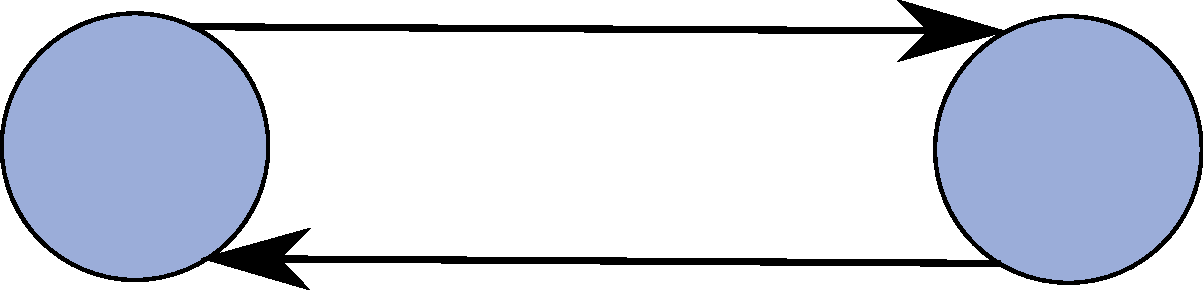
\includegraphics[width=1.78646in,height=0.38583in]{figs/mutual-cooperation-graph}
    \caption{A graph representing a situation of mutual cooperation. An arrow from A to B indicates
    that A can benefit B.}
    \label{mutual-cooperation-graph}
\end{figure}

In mutual relations like this, it is possible to apply causal
cooperation, although only if the interaction is
\href{https://en.wikipedia.org/wiki/Prisoner\%27s_dilemma\#The_iterated_prisoner.27s_dilemma}{repeated}
-- i.\,e. if my choice causally influences the other agent's
choice\footnote{Note that in causal cooperation, cooperative or
  uncooperative behavior
  \href{https://en.wikipedia.org/wiki/Reciprocity_(evolution)\#Indirect_reciprocity}{may}
  also causally affect bystanders and thus increase the probability that
  I can establish cooperation with them in the future.}, and then the
other agent's choice can causally influence my choice, etc.\footnote{Throughout
  this treatment, the graphs do not represent time and repetition. This
  could be done by taking the given static graphs and ``unfolding
  through time'', similar to how it is done when
  \href{https://en.wikipedia.org/wiki/Backpropagation_through_time}{applying
  backpropagation to recurrent neural networks}. The resulting graph
  may then resemble a
  \href{https://en.wikipedia.org/wiki/Unified_Modeling_Language\#Interaction_diagrams}{UML
  interaction diagram}.} (For introductions, see, e.\,g.
  Axelrod \citeyear{Axelrod2006-ci}, Trivers \citeyear{Trivers1971-rb}, Fehr and Gächter
  \citeyear{Fehr1999-pd}, Dawkins \citeyear{Dawkins1976-cd}, Taylor \citeyear{Taylor1987-wn}, and
  Buss \citeyear{Buss2015-kp}.)

Superrational cooperation also works in the above scheme, although
repetition is not required. The
\href{https://en.wikipedia.org/wiki/Prisoner\%27s_dilemma}{prisoner's
dilemma}
(\href{http://plato.stanford.edu/entries/prisoner-dilemma/\#PDRepCauDecThe}{with
replicas} or twins) is one example of this sort of problem.

\subsubsection{Circular cooperative structures and indirect causal
reciprocity}\label{circular-cooperative-structures-and-indirect-causal-reciprocity}

In principle, it is possible to establish causal cooperation even in
cases where the two agents cannot directly benefit each other, provided
there is a repeated causal link from my own decision to the decision of
the agent who can benefit or hurt me, such that I can in some way reward
cooperation and punish defection. As an example, consider the following
variation of Hofstadter's donation game:

\begin{quote}
\textbf{Donation circle.} Omega has a list of 6 participants. The list
is
\href{https://en.wikipedia.org/wiki/Linked_list\#Circular_Linked_list}{circular},
meaning that every participant has a successor. Omega sends each
participant a letter, asking them to respond with single letter `C' (for
cooperate) or `D' (for defect) without communicating with each other. It
explains that by sending in `C', participants can increase their
successor's payoff by \$5. By sending in `D', they can increase their
own payoff by \$2. As usual, the participants are told that they are all
rational or that they use similar decision mechanisms. Every participant
only cares about the balance of her own bank account, and not about
Omega's or that of the other 6 participants. Upon receiving the letter,
should you cooperate or defect?

\textbf{Iterated donation circle.} Like the circular donation game, only
that the game is played many times (the exact number of times being
unknown to the players). In every round, each participant is informed of
their predecessor's past choices before deciding whether to send in `C'
or `D'.
\end{quote}

Circular structures such as these can be represented by graphs such as
the one in Figure \ref{circular-cooperation-graph}.

\begin{figure}[h!]
    \centering
    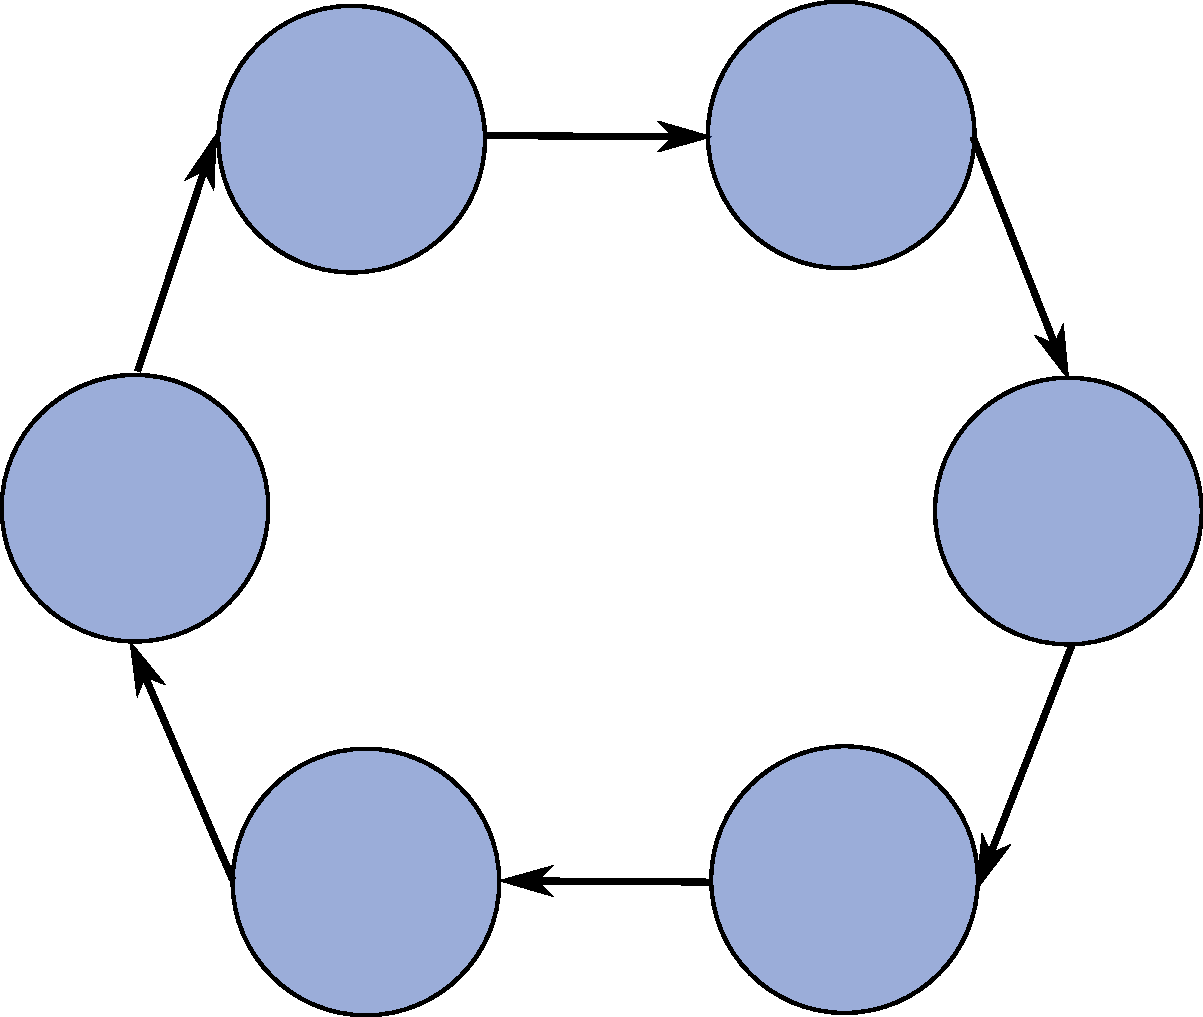
\includegraphics[width=1.68409in]{figs/circular-cooperation-graph}
    \caption{A circular cooperation graph
representing cooperation schemes of the sort used in the Donation
circle. Again, an arrow from A to B indicates that A can benefit B.}
    \label{circular-cooperation-graph}
\end{figure}

Because each of the agents can causally (through the other agents)
affect their predecessor, the iterated version of this problem could
still, in principle, motivate causal cooperation. For example, one
\href{https://en.wikipedia.org/wiki/Nash_equilibrium}{Nash
equilibrium} consists in everyone playing
\href{https://en.wikipedia.org/wiki/Tit_for_tat}{tit for tat}.
This Nash equilibrium is even
\href{https://en.wikipedia.org/wiki/Nash_equilibrium\#Stability}{stable},
in the sense that one player diverging from tit for tat with a very
small probability still leaves everyone else best off if they continue
to use tit for tat.

However, the same Nash equilibrium is also hard to achieve and unstable
in a different sense, as it requires all 6 participants to use the same
kind of strategy. Your response to your predecessor's cooperation is
mediated by multiple other agents. If only one of them does not
propagate your response correctly, the causal path from you to your
predecessor is disrupted, leaving neither of you with a causal
motivation to cooperate.

For superrationality-based considerations, on the other hand, neither
repetition nor the length of the causal path from one participant's
cooperation to her predecessor are relevant. Instead, superrational
cooperation only on the correlations between single pairs of agents.
Hence, while the significance of causal cooperation in the Donation
circle diminishes with every additional participant, the benefits from
superrational cooperation remain constant regardless of how many players
are involved.

\hypertarget{hierarchies-and-acyclic-graphs}{\subsubsection{Hierarchies
and acyclic graphs}\label{hierarchies-and-acyclic-graphs}}

In an extreme case, there would be no causal path whatsoever from one
participant's cooperation to that of his predecessor, making causal
cooperation lose its entire appeal to the rational agent. Superrational
cooperation, on the other hand, may still be applicable (cf.
Drescher \citeyear{Drescher2006-ky}; see
section \ref{gary-drescher-on-superrationality}).

Consider the following variant of the donation game:

\begin{quote}
\textbf{Donation ladder.} Once more, Omega has a long list of
participants, albeit a regular linear one this time. Omega sends all of
them a letter, asking them to respond with a single letter `C' (for
cooperate) or `D' (for defect) without communicating with each other. It
explains that by sending in `C', participants can increase their
successors' payoffs by \$5. The first person on the list cannot benefit
from the cooperative behavior of others, and the last participant's
choice has no effect on the others. Omega writes that each player can
increase their own payoff by \$2 if they defect. Participants do not
know their position on the list, and are once again told that they all
use similar decision algorithms. Every participant only cares about the
balance of their own bank account, and not about Omega's or that of the
other participants. Upon receiving the letter, should you cooperate or
defect?
\end{quote}

Figure \ref{donation-ladder} illustrates the donation
ladder.

\begin{figure}[h!]
    \centering
    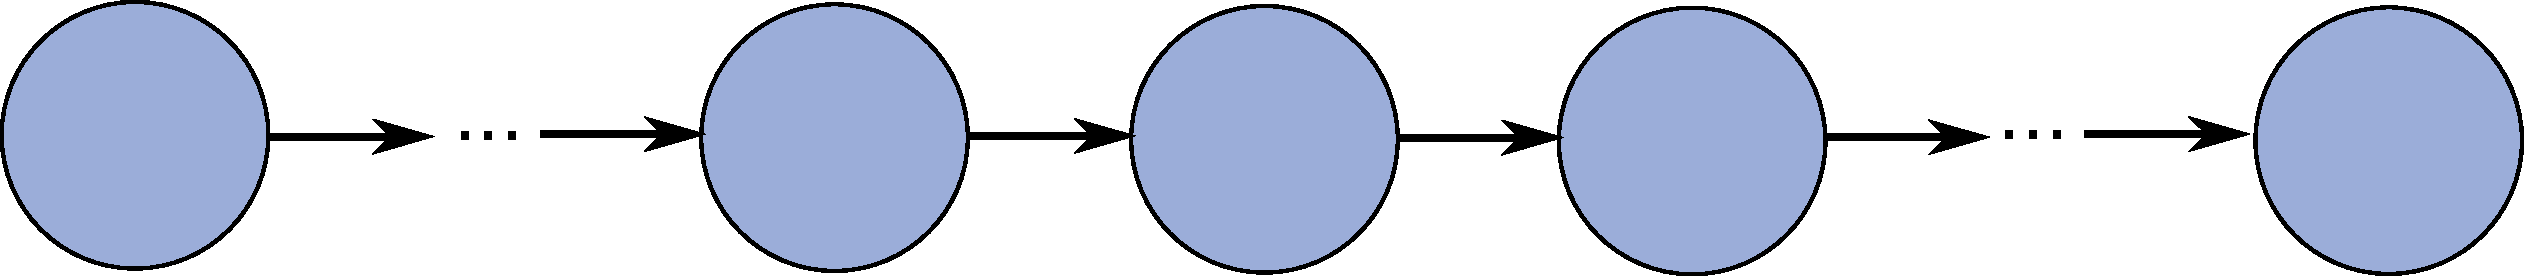
\includegraphics[width=5.19271in,height=0.49167in]{figs/donation-ladder}
    \caption{A linear cooperation graph (graph theoretically
speaking, a 1-ary tree) representing schemes of cooperation like that in
the donation ladder. An arrow from A to B indicates that A can benefit
B.}
    \label{donation-ladder}
\end{figure}

Again, the nodes represent participants and an arrow from A to B
indicates that A can bring causal benefits to B.

In such a cooperation scheme, causal cooperation cannot be established
even if the problem is iterated, whereas the superrationality mechanism
is just as reliable as in the other examples. Because the list is long,
I probably have a predecessor; if I cooperate, then my predecessor --
who is in a position similar to mine -- will probably make the same
choice. Cooperation thus informs me (or logically determines) that I am
likely to gain \$5, whereas defection only gives me \$2.

We can see this linear hierarchy of agents in practice among the
different versions of an agent at various points in time. For example, I
can causally affect the welfare of future versions of myself, but if I
only (or primarily) care about my present experiences, they can never
reward me in return. However, I could try to benefit future versions of
myself to make it more likely that past versions of me have behaved
nicely toward myself. More discussion with references to the literature
is given by Drescher (\cite{Drescher2006-ky}, section 7.3.4).

Linear cooperation hierarchies come with a twist, however. Consider the
following variant of the Linear hierarchical donation game:

\begin{quote}
\textbf{Donation ladder with known position.} Identical to the linear
hierarchical donation game, only that participants know their position
in the list when they make their decision.
\end{quote}

A participant in the middle of the list may wonder how his situation
differs from the regular donation ladder -- after all, his predecessor
on the list is in almost the same situation as he is. Assuming the
conditions for superrationality are satisfied, their decisions should
still correlate. Hence, if he cooperates, should we assume that his
predecessor is likely to do the same?

Not necessarily. The problem lies in the beginning of the list. The
first person -- let us call her No. 1 -- will have no predecessor and
thus no predecessor whose decision she could acausally influence, in
effect giving her no reason to cooperate. Given this, No. 1 should
defect (that is, unless she is already updateless; more on this below).

Unfortunately, this puts No. 2 in a similar position. Realizing that No.
1 will defect, there is nobody left to benefit \emph{him}. No. 3 will,
in turn, reason that No. 2 expects No. 1 to defect, which means that No.
2 will also defect, leading No. 3 to defect as well\ldots{} and so on,
propagating down the entire list. You may notice that this propagating
defection effect is analogous to the reason why
\href{https://en.wikipedia.org/wiki/Prisoner\%27s_dilemma\#The_iterated_prisoner.27s_dilemma}{standard
game theory recommends to defect in the iterated prisoner's dilemma when
the number of rounds is known}\footnote{Even in the iterated prisoner's
  dilemma, this answer -- supported by
  \href{https://en.wikipedia.org/wiki/Backward_induction}{backward
  induction} --
  \href{http://lesswrong.com/lw/to/the_truly_iterated_prisoners_dilemma/n23}{is
  often seen as unsatisfactory}. Other examples of paradoxes caused by
  backward induction are the
  \href{https://en.wikipedia.org/wiki/Chainstore_paradox}{chainstore
  paradox}, the
  \href{https://en.wikipedia.org/wiki/Traveler\%27s_dilemma}{traveler's
  dilemma}, the
  \href{https://en.wikipedia.org/wiki/Unexpected_hanging_paradox}{unexpected
  hanging paradox}, the
  \href{https://en.wikipedia.org/wiki/The_Bottle_Imp\#Bottle_Imp_paradox}{Bottle
  Imp paradox}, the
  \href{https://en.wikipedia.org/wiki/Centipede_game}{centipede
  game}, the
  \href{https://en.wikipedia.org/wiki/Interesting_number_paradox}{interesting
  number paradox}, the
  \href{https://en.wikipedia.org/wiki/Guess_2/3_of_the_average}{guess
  2/3 of the average game}. A good introduction is given by
  \href{http://www.cs.virginia.edu/~robins/The_Travelers_Dilemma.pdf}{Basu
  (2007)}. For further references, see Basu \citeyear{Basu1994-xk}.}.

Once more, we find that lack of knowledge is evidential power. For one,
if the participants did not know their positions, they would all
cooperate -- and thus be more successful. If everyone could precommit to
cooperation before learning about their position, they would do so.
Again, cooperation
\href{https://casparoesterheld.com/2016/11/21/thoughts-on-updatelessnes/}{can}
be maintained if all the agents are updateless in the first place (see
section
\ref{lack-of-knowledge-is-evidential-power-part-ii-taking-a-step-back}, cf.
\cite{Drescher2006-ky}, chapter 7.2.2). If all of this is not the
case, nothing can change the fact that at least No. 1
``\href{https://wiki.lesswrong.com/wiki/Rationality_is_systematized_winning}{wins}
by defecting once she knows her position on the list.

Secondly, thinking about the other agents' decisions can be dangerous.
No. 42 defects solely because he thinks about what the preceeding 41
participants decide. Knowing what the other agents think is thus harmful
for some not-yet-updateless decision theories. Hence, similar to how it
is wise to remain ignorant about your position in the list, many
decision theories would recommend not thinking about what the other
agents will do. If the players are human, then No. 1 may not be able to
refrain from realizing that he wins by defecting. Perhaps No. 2 cannot
refrain from realizing that No. 1's situation is different and his
decision therefore independent of hers. However, participants with
two-figure positions may be able to refrain and go with the reasoning
originally presented: whatever I choose, my predecessor will probably
choose the same, as his situation is similar to mine. If I just go ahead
without thinking about the ``chain of defection'' initiated by No. 1,
then people with similar numbers are probably going to do the same.

The linear structure can be generalized to non-linear hierarchical
cooperation schemes. Consider the following variant of the donation
game:

\begin{quote}
\textbf{Donation tree.} Omega has a long list of participants again. It
sends all of them a letter, asking them to respond with a single letter
`C' (for cooperate) or `D' (for defect) without communicating with each
other. Omega explains that by sending in `C', participants can increase
the payoff of at least 3 participants down the list by \$2 each. For
example, if the 4th participant chooses to cooperate, this benefits a
subset of the participants in positions 5, 6, etc. but not the previous
3 participants. The cooperation of the last few participants has little
to no effect. By sending in `D' participants can increase their own
payoff by \$5. Participants do not know their position on the list or
whom they could benefit. As usual, they are told that they all use
similar decision mechanisms. Every participant only cares about the
balance of their own bank account, and not about Omega's or the other
participants'. Upon receiving the letter, should a participant cooperate
or defect?
\end{quote}

In general, we can represent such hierarchical versions of the donation
game using
\href{https://en.wikipedia.org/wiki/Directed_acyclic_graph}{directed
acyclic graphs} like the one in Figure \ref{donation-DAG}.

\begin{figure}[h!]
    \centering
    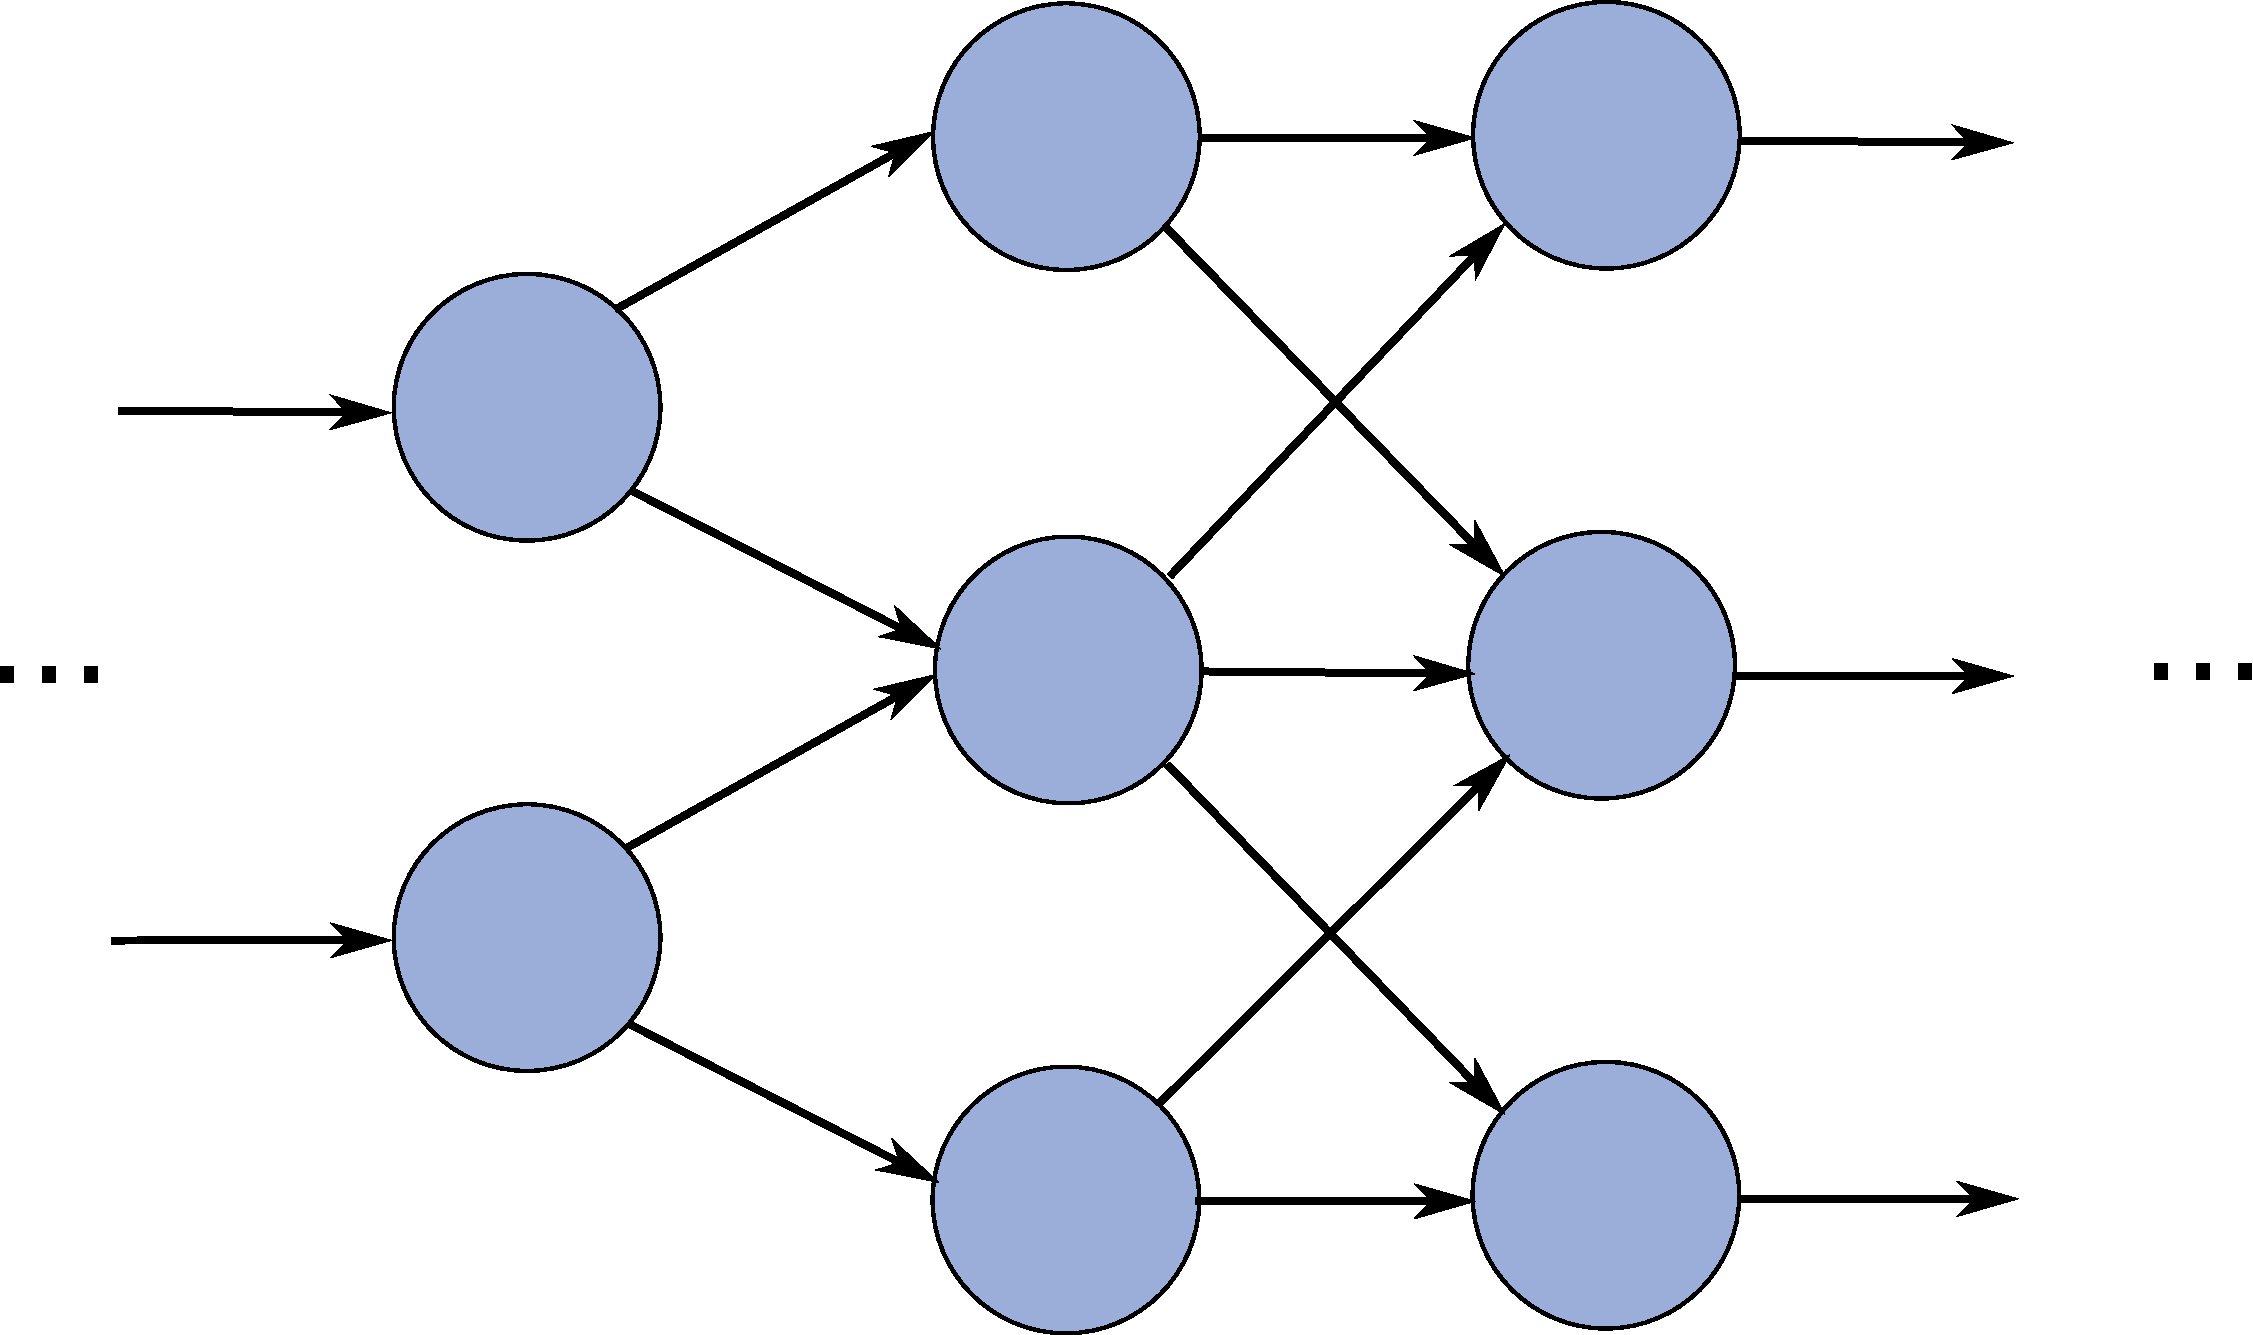
\includegraphics[width=3.98958in,height=2.05728in]{figs/donation-DAG}
    \caption{A directed acyclic graph representing the schemes of cooperation like that of the
    Hierarchical donation game.}
    \label{donation-DAG}
\end{figure}

If participants knew their respective positions in the list, the
considerations outlined for the Donation ladder with known position
would apply analogously.

In practice, such hierarchies may be hierarchies of power. Some agents
are ``lexically'' more powerful than others, such that cooperation can
only be beneficial in one direction -- the less powerful have no way of
helping the more powerful, while the powerful can help less powerful
ones much more cheaply. As a perhaps paradigmatic example, consider a
standard science-fiction scenario:

\begin{quote}
\textbf{Intergalactic relations.} The universe contains many
civilizations. Although they all followed similar evolutionary
trajectories, each civilization developed at different times on
different planets in different parts of the universe, and thus differ
drastically in their levels of sophistication. Most civilizations
eventually decided to conceal themselves to some extent, so no one knows
which of the civilizations is the most powerful. You are the leader of a
civilization, and one day, you encounter a comparably primitive
civilization for the first time. According to your advisors, it appears
that, this other civilization has not even managed to harness the energy
of their local star, they still suffer from diseases that your
civilization's nano-devices could cure in an instant, and so forth. Your
advisors, citing the other civilization's apparently laughable defense
systems, recommend that you destroy them and use their resources to
further your own goals. Should you follow your advisors' recommendation?
\end{quote}

Once again, causal reasoning may suggest that you should. By now,
though, it should be clear that there are good reasons to ignore your
advisor's recommendation if you believe there is a sufficiently strong
correlation between your and the other civilizations.

Note that one reason for civilizations to conceal themselves might be to
induce a lack of knowledge about their relative positions within the
hierarchy. If we remain hidden, other civilizations will be more likely
to do the same, so neither we nor they would know who has the upper hand
in a potential confrontation. On the other hand, if all civilizations
loudly boasted their power, the most powerful civilization would realize
its dominance and consequently have no reason to be friendly to the
others -- absent precommitment, the use of updateless decision theory,
and the like.

Another example of such power hierarchies is that of simulations.
Simulators can causally influence the simulated in any way they want,
but the simulated can do little to causally affect the simulators (e.\,g.,
by
\href{https://foundational-research.org/how-the-simulation-argument-dampens-future-fanaticism\#Our_simulated_copies_can_still_impact_the_far_future_by_helping_our_simulators}{affecting
the outcomes of the simulation} or its computational demands). We will
discuss this more in section
\ref{simulations}.

The following example may be typical of the hierarchies in
multiverse-wide superrationality (MSR):

\begin{quote}
\textbf{Computable consequentialists.} Meet Luca, who believes that
consciousness cannot arise from
\href{https://en.wikipedia.org/wiki/Computability}{classical
computation} alone.\footnote{Two classes of hypotheses in this space
  are
  \href{https://en.wikipedia.org/wiki/Mind\%E2\%80\%93body_dualism\#Substance_dualism}{substance
  dualism} and the
  \href{https://en.wikipedia.org/wiki/Quantum_mind}{quantum
  mind}. Both have a few prominent proponents but are nonetheless
  fringe positions in philosophy of mind. I concur with the majority and
  am skeptical of both hypotheses.} He is also a consequentialist and
primarily cares about conscious experiences. Through the
\href{https://en.wikipedia.org/wiki/Mathematical_universe_hypothesis}{\emph{writings}
\emph{of Tegmark}}, Luca has come to believe that many computable
universes might exist in parallel to ours. However, since these
computable universes do not contain anything that he would call a
conscious experience, Luca does not care about what goes on inside them.
He does, however, enjoy thinking about their inhabitants as an
intellectual exercise, and this has led him to the conclusion that they
\emph{can} reason about Newcomb-like scenarios in a human-like way even
though they are insentient. After all, neither calculating conditional
probabilities nor operating on causal graphs requires sentience. Using
the supercomputer in his basement, Luca has also come up with a number
of predictions about the values held by consequentialists in the
computable universes -- let us call them the computable
consequentialists (CCs) -- a feat more difficult to achieve for
incomputable worlds. He has even discovered a number of ways to benefit
the CCs' values in our universe, all at a very low cost to his own
values. While Luca himself does not care about computable universes, he
sees no reason for the CCs not to care about worlds that are
computationally more powerful than their own. Given that the CCs cannot
do anything for Luca in their world, however, is it rational for Luca to
be friendly to the CCs' values?
\end{quote}

Again, Luca does indeed have a reason to do so. If he benefits the CCs,
other agents -- including ones whom Luca cannot benefit -- are more
likely to realize Luca's goals in other parts of the multiverse.

The ability to help can also come from knowing about the other agents.
Consider the following example:

\begin{quote}
\textbf{Simple-world ignorance.} Imagine a multiverse in which many
different sets of laws of physics are realized. Some of the universes
have very simple, parameterless, and easily understood basic laws, like
\href{https://en.wikipedia.org/wiki/Conway\%27s_Game_of_Life}{Conway's
Game of Life}. Others have far more complicated rules. The inhabitants
of the more complex universes may thus have more reason to believe in
the multiverse than the inhabitants of the simple universes. In the
complex universe, the multiverse hypothesis is attractive because it is
\href{http://lesswrong.com/lw/jp/occams_razor/}{simpler} than the
hypothesis that only their universe exists (cf.
\href{ftp://ftp.idsia.ch/pub/juergen/everything.pdf}{Schmidhuber
1997}). In the simple universe, on the other hand, the multiverse
hypothesis may be more complex than the hypothesis that only their
universe exists. Consequently, the inhabitants of the simple universes
may adopt superrationality but only apply it toward other inhabitants of
their universe. Let us assume that the values of the folks from the
simple universes differ significantly from those of the inhabitants of
the more complex universes. Should the inhabitants of the complex
universes help the values of those from the simple universes?
\end{quote}

In this scenario, as with the previous ones in this section, I think
that the superrationalists from the more complex universes have good
reason to help the superrationalists from the simpler universes, as this
makes it more probable that the former will receive help from other
agents, including ones that \emph{they} cannot help. For example, there
may be many value systems that \emph{they} (the inhabitants of the
complex universes) do not know about (for reasons other than the
Kolmogorov complexities of different multiverses).

I think this particular scenario may well be relevant in our multiverse.
More generally, some parts of the multiverse may contain different clues
about the existence of other superrational agents. For example, some
might live in parts of the universe from which it looks as though life
is much rarer than it actually is, whereas others may discover that they
are not alone as soon as they look through a telescope for the first
time. In addition, while a superrational agent may be able to use some
theory of physics to infer the existence of other agents, he or she may
be unable to infer the existence of some particular value system.

\hypertarget{only-helping-superrational-cooperators-helps-you-superrationally}{\subsubsection{Only
helping superrational cooperators helps you
superrationally}\label{only-helping-superrational-cooperators-helps-you-superrationally}}

Cooperation usually excludes agents who are known to be unable to
reciprocate. Yet as we learned from the Donation tree and Intergalactic
relations, superrationality does allow for cooperation with
non-reciprocating agents if helping them makes it more likely that other
agents help us.

There is, however, at least one limitation on the set of our
beneficiaries that comes without negative side-effects. We can exclude
from superrational cooperation all agents who do not cooperate
superrationally at all. After all, every superrational cooperator knows
that this exclusion will not affect her, and the exclusion appears to be
symmetrical among all superrational agents. That is, it makes it more
likely that other superrational cooperators make the same choice (rather
than incurring some other limitation that excludes us).

It seems risky to place any stronger limitation on the set of our
beneficiaries, since this would give us reason to fear exclusion by
other agents (cf. \cite{Drescher2006-ky}), as we have
seen in section
\ref{hierarchies-and-acyclic-graphs}. If we so much as try to look for rules of
exclusivity that benefit us at the expense of other superrational
agents, we have reason to believe that others will do so as well.

Of course, superrationality and correlation between decisions are not
binary properties, so neither is the limitation drawn above. For
example, two artificial intelligences explicitly based on the same
decision theory may correlate more than two (non-copied) humans, even if
both have some incentive to cooperate. The stronger the correlation
between us and some other agent, the more we will benefit
superrationally from helping them (cf.
\cite{Drescher2006-ky}). To illustrate this, consider a
one-shot prisoner's dilemma-like situation in which two very similar
agents can simultaneously decide whether to give the other one some
reward \(b_{\text{other}}\) or to walk away with a smaller reward
\(b_{u}\) for themselves. The cooperation graph looks like this:

\begin{figure*}[h!]
    \centering
    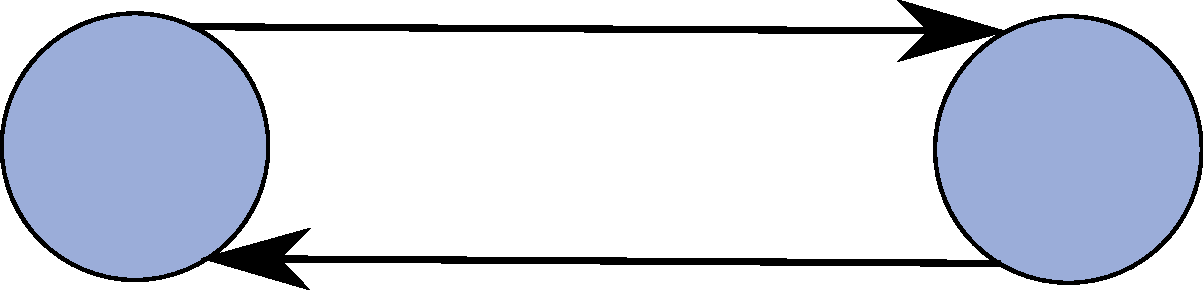
\includegraphics[width=1.78in]{figs/mutual-cooperation-graph}
\end{figure*}

Now, imagine the two agents are perfectly correlated, i.\,e. they always
make the same decision. If this is the case, both agents should
cooperate whenever
\begin{equation}
    b_{\text{other}} > b_{u}.
    \label{eq:condition_coop}
    % previously (*)
\end{equation}

Now consider a situation in which the correlation between the two agents
is weaker. Then, in EDT terms, they should cooperate if cooperation (C)
is higher in expected value than defection (D), i.\,e. if
$$
\mathrm{E}\lbrack C\rbrack > \mathrm{E}\lbrack D\rbrack.
$$

Using conditional probabilities, we can reformulate this as
$$
P(C\mid C) \cdot b_{\text{other}} > P(C\mid D) \cdot (b_{\text{other}} + b_{u}) + P(D\mid D) \cdot b_{u} =
P(C\mid D) \cdot b_{\text{other}} + b_{u},
$$
where, for example, \(P(C\mid C)\) is the probability that the other side
cooperates conditional on my cooperation. Solving for \(b_{\text{other}}\) yields
\begin{equation}
    b_{\text{other}} > \frac{b_{u}}{P(C\mid C) - P(C\mid D)},
    \label{eq:solve_p}
    % previously (**)
\end{equation}
where \(P(C\mid C) - P(C\mid D)\) can be interpreted as quantifying how much
more likely my cooperation makes the other's cooperation. Because there
is at least some correlation, the term is always greater than 0. If the
correlation is perfect, then \(P(C\mid C) = 1\) and \(P(C\mid D) = 0\), such
that we get Eq.~\eqref{eq:condition_coop} as a special case of Eq.~\eqref{eq:solve_p}. If the correlation is less
than perfect, then \(b_{a} > b_{s}\) may not be enough. For example, if
\(P(C\mid C) = 0.8 = P(D\mid D)\) (such that whatever one agent does, the other
agent is 80\% likely to do the same), then it must hold that
$$
b_{a} > \frac{b_{s}}{P(C\mid C) - P(C\mid D)} = \frac{b_{s}}{0.8 - 0.2} = \frac{5}{3}b_{s}.
$$
Thus, the threshold for cooperation increases as the correlation between
the two agents decreases.

If the cooperation graphs become more complicated, then so do
calculations like those above. Further research is needed to find out
whether the above result -- that benefitting agents with stronger
correlation is more important -- holds true more generally. One
interesting question is to what extent superrationalists would form
clusters based on correlation strength. This is especially relevant if
we believe the correlations to be especially strong among agents with
the same value system.

\hypertarget{cheating-signaling-and-half-heartedness}{\subsection{Cheating,
signaling, and
half-heartedness}\label{cheating-signaling-and-half-heartedness}}

Causal and superrational cooperation differ in another important
respect. In causal cooperation, the benefit of cooperative behavior
comes from how other agents will react to one's own cooperative
acts.\footnote{For references to the literature, see section
  \ref{schemes-of-causal-cooperation}.} To facilitate cooperation, each agent may
commit to reward cooperative and punish uncooperative behavior. In this
way, they can motivate each other to cooperate. But seeing as behavior
can only be rewarded or punished if it is observed at all, causal
cooperation often ends up focusing heavily on signalling. If you can
save costs by merely pretending (in a convincing way) to have
cooperated, then that is the rational thing to do from a causal
perspective. Conversely, if you can help someone without them knowing
about it, you have no causal reason to do so. There are many practical
examples of this, such as the tendency for governments to make a big
deal out of international agreements or cooperative acts, even if the
object-level gain is minor.

Since the mechanism of superrational cooperation is different from that
of regular causal cooperation, prioritization within it should be
different, too. Specifically, superrational cooperation is beneficial
not because others reciprocate one's cooperative acts, but because our
(cooperative) decisions correlate with those of others. This means that
we should sincerely attempt to maximize for benefits to other value
systems, because this correlates with others doing the same, which in
turn maximizes our own benefits.

We are used to thinking about cooperation in causal terms, i.\,e. about
how a certain cooperative act may in the end pay us back causally and in
this universe. If we think about superrational cooperation in this old
mindset, we may be tempted to propose measures that are critically
suboptimal from a superrational standpoint. For instance, one may adopt
a ``compartmentalized good will'', talking at length about cooperation
without actually trying to maximize for other agents' goal achievement,
or spend time thinking about how the others might cheat us.

However, all of these correlate with other superrational agents in the
multiverse wasting effort on these exact same things. With superrational
cooperation, only sincere attempts at improving other agents' value
systems correlate with the same behavior in others, and thus with the
optimal consequences. Hence, there is no way to ``game the system'' or
to get benefits without honestly paying for them.
